

%% 
%% Copyright 2007-2020 Elsevier Ltd
%% 
%% This file is part of the 'Elsarticle Bundle'.
%% ---------------------------------------------
%% 
%% It may be distributed under the conditions of the LaTeX Project Public
%% License, either version 1.2 of this license or (at your option) any
%% later version.  The latest version of this license is in
%%    http://www.latex-project.org/lppl.txt
%% and version 1.2 or later is part of all distributions of LaTeX
%% version 1999/12/01 or later.
%% 
%% The list of all files belonging to the 'Elsarticle Bundle' is
%% given in the file `manifest.txt'.
%% 
%% Template article for Elsevier's document class `elsarticle'
%% with harvard style bibliographic references

%\documentclass[preprint,12pt,authoryear]{elsarticle}
%\documentclass[3p, 12pt,authoryear]{elsarticle}
\documentclass[final, 3p, times, authoryear]{elsarticle}

%% Use the option review to obtain double line spacing
%% \documentclass[authoryear,preprint,review,12pt]{elsarticle}

%% Use the options 1p,twocolumn; 3p; 3p,twocolumn; 5p; or 5p,twocolumn
%% for a journal layout:
%% \documentclass[final,1p,times,authoryear]{elsarticle}
%% \documentclass[final,1p,times,twocolumn,authoryear]{elsarticle}
%% \documentclass[final,3p,times,authoryear]{elsarticle}
%% \documentclass[final,3p,times,twocolumn,authoryear]{elsarticle}
%% \documentclass[final,5p,times,authoryear]{elsarticle}
%% \documentclass[final,5p,times,twocolumn,authoryear]{elsarticle}

%% For including figures, graphicx.sty has been loaded in
%% elsarticle.cls. If you prefer to use the old commands
%% please give \usepackage{epsfig}

%% The amssymb package provides various useful mathematical symbols
\usepackage{amssymb}
%% The amsthm package provides extended theorem environments
\usepackage{amsmath,amsthm}

%% The lineno packages adds line numbers. Start line numbering with
%% \begin{linenumbers}, end it with \end{linenumbers}. Or switch it on
%% for the whole article with \linenumbers.
%% \usepackage{lineno}

\usepackage{hyperref}
\usepackage{multirow}
\usepackage{pgfplots}
\usepackage{arydshln}
\usepackage{paralist}
\usepackage{multicol}

%% Comments
\newif\ifcomments\commentstrue

\ifcomments
\newcommand{\authornote}[3]{\textcolor{#1}{[#3 ---#2]}}
\newcommand{\todo}[1]{\textcolor{red}{[TODO: #1]}}
\else
\newcommand{\authornote}[3]{}
\newcommand{\todo}[1]{}
\fi

\newcommand{\wss}[1]{\authornote{blue}{SS}{#1}} %Spencer Smith
\newcommand{\jc}[1]{\authornote{red}{JC}{#1}} %Jacques Carette
\newcommand{\zm}[1]{\authornote{magenta}{MN}{#1}} %Zahra Motamed
\newcommand{\pmm}[1]{\authornote{cyan}{AD}{#1}} %Peter Michalski

\newcommand{\notdone}[1]{\textcolor{red}{#1}}
\newcommand{\done}[1]{\textcolor{black}{#1}}

% For easy change of table widths
\newcommand{\colZwidth}{1.0\textwidth}
\newcommand{\colAwidth}{0.24\textwidth}
\newcommand{\colBwidth}{0.76\textwidth}
\newcommand{\colCwidth}{0.28\textwidth}
\newcommand{\colDwidth}{0.72\textwidth}
\newcommand{\colEwidth}{0.33\textwidth}
\newcommand{\colFwidth}{0.67\textwidth}
\newcommand{\colGwidth}{0.5\textwidth}
\newcommand{\colHwidth}{0.28\textwidth}

\newcounter{comnum} %Commonality Number
\newcommand{\cthecomnum}{C\thecomnum}
\newcommand{\cref}[1]{C\ref{#1}}

\newcounter{varnum} %Variability Number
\newcommand{\vthevarnum}{V\thevarnum}
\newcommand{\vref}[1]{V\ref{#1}}

\newcounter{parnum} %Parameter of Variation Number
\newcommand{\ptheparnum}{P\theparnum}
\newcommand{\pref}[1]{P\ref{#1}}

\newcommand{\CC}{C\nolinebreak\hspace{-.05em}\raisebox{.4ex}{\small\bf
+}\nolinebreak\hspace{-.10em}\raisebox{.4ex}{\small\bf +}}

\journal{???}

\begin{document}

\begin{frontmatter}

%% Title, authors and addresses

%% use the tnoteref command within \title for footnotes;
%% use the tnotetext command for theassociated footnote;
%% use the fnref command within \author or \affiliation for footnotes;
%% use the fntext command for theassociated footnote;
%% use the corref command within \author for corresponding author footnotes;
%% use the cortext command for theassociated footnote;
%% use the ead command for the email address,
%% and the form \ead[url] for the home page:
%% \title{Title\tnoteref{label1}}
%% \tnotetext[label1]{}
%% \author{Name\corref{cor1}\fnref{label2}}
%% \ead{email address}
%% \ead[url]{home page}
%% \fntext[label2]{}
%% \cortext[cor1]{}
%% \affiliation{organization={},
%%            addressline={}, 
%%            city={},
%%            postcode={}, 
%%            state={},
%%            country={}}
%% \fntext[label3]{}

\title{State of the Practice for Lattice Boltzmann Method Software}

%% use optional labels to link authors explicitly to addresses:
%% \author[label1,label2]{}
%% \affiliation[label1]{organization={},
%%             addressline={},
%%             city={},
%%             postcode={},
%%             state={},
%%             country={}}
%%
%% \affiliation[label2]{organization={},
%%             addressline={},
%%             city={},
%%             postcode={},
%%             state={},
%%             country={}}

\author[CAS]{Spencer Smith}
\author[CAS]{Peter Michalski}
\author[CAS]{Jacques Carette}
\author[ME]{Zahra Motamed}

\affiliation[CAS]{organization={McMaster University, Computing and Software
Department},%Department and Organization
            addressline={1280 Main Street West}, 
            city={Hamilton},
            postcode={L8S 4K1}, 
            state={Ontario},
            country={Canada}}

\affiliation[ME]{organization={McMaster University, Mechanical Engineering},%Department and Organization
            addressline={1280 Main Street West}, 
            city={Hamilton},
            postcode={L8S 4K1}, 
            state={Ontario},
            country={Canada}}

\begin{abstract}

    We analyze the state of software development practice for Lattice Boltzmann
    solvers by quantitatively and qualitatively measuring and comparing 24
    software packages for 10 software qualities (installability, correctness/
    verifiability, reliability, robustness, usability, maintainability,
    reusability, understandability, visibility/transparency and
    reproducibility). Our reproducible analysis method employs a measurement
    template (containing 103 measures that are manually and automatically
    extracted from the project repository) and developer interviews (consisting
    of a set of 20 questions). From the measurement results, we ranked the
    software using the Analytic Hierarchy Process (AHP), a multi-criteria
    decision making method appropriate for cases with a mix of qualitative and
    quantitative factors. Our ranking was roughly consistent with ranking the
    repositories by the number of GitHub stars, although the number one project
    by star count (Sailfish) is ranked 9th by our methodology. Our top three
    packages were Ludwig, ESPResSo, and Palabos (all in the top 10 by star
    count). We interviewed 4 developers to gain insight into their current pain
    points. Identified challenges include lack of development time, lack of
    funding, and difficulty with ensuring correctness.  Based on our assessment,
    we make the following recommendations for current and future LBM projects:
    provide a detailed user manual and tutorials, explicitly state the limits of
    the software, use user-friendly programming languages, consider a peer
    review process, communicate development and contribution information, and
    use continuous integration and project management tools.

\end{abstract}

%%Graphical abstract
%\begin{graphicalabstract}
%\includegraphics{grabs}
%\end{graphicalabstract}

%%Research highlights
%\begin{highlights}
%\item Research highlight 1
%\item Research highlight 2
%\end{highlights}

\begin{keyword}
	Lattice Boltzmann Method (LBM), scientific computing, software engineering,
	software quality, Analytic Hierarchy Process
\end{keyword}

\end{frontmatter}

%% \linenumbers

\section{Introduction}

We analyze the development of Computational Fluid Dynamics (CFD) software
packages that use the Lattice Boltzmann Method (LBM). LBM packages form a family
of algorithms for simulating single-phase and multiphase fluid flows, often
incorporating additional physical complexities \citep{chen1998lattice} such as
reflective and non-reflective boundaries. They consider the behaviour of a
collection of particles as a single unit at the mesoscopic scale, between the
nanoscopic and microscopic scales. LBM solvers predict the positional
probability of a collection of particles moving through a lattice structure
following a two step process: i) streaming, where the particles
move along the lattice via links; and, ii) colliding, where energy and
momentum is transferred among particles that collide \citep{bao2011lattice}. As
an example of the output of LBM, Figure~\ref{circularflow} presents the streamlines of
converged flow past a stationary circular cylinder with varying Reynolds numbers.
\wss{Zahra might have a better example?  A journal publication isn't likely
going to accept a figure produced for another paper.}  LBM has several
advantages over conventional CFD methods, including a simple calculation
procedure, improved parallelization, and robust handling of complex geometries
\citep{ganji2015application}.

\begin{figure}[h!]
	\begin{center}
		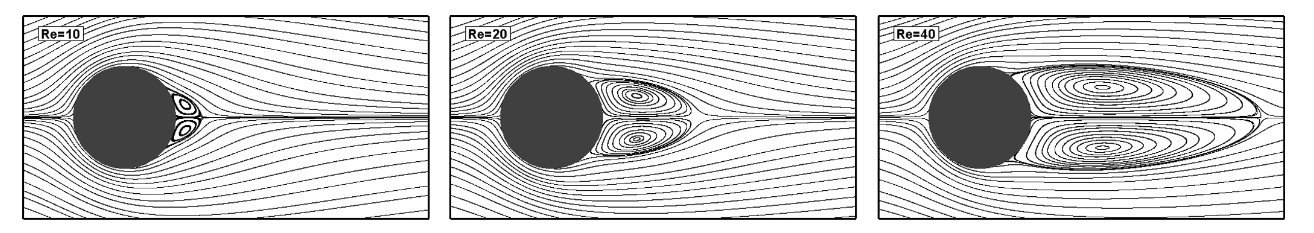
\includegraphics[width=0.7\textwidth]{./figures/circularflow}
		\caption{Streamlines of flow past a stationary circular cylinder at
		Reynolds number = 10, 20, and 40 \citep{chen2021phase}}
		\label{circularflow}
	\end{center}
\end{figure}

A small sample of important applications of LBM include the following: designing
fuel cells \citep{ZhangEtAl2018}, modelling groundwater flow
\citep{AnwarAndSukop2009}, and analyzing the flow of blood in the cardiovascular
system \citep{SadeghiEtAl2020}.  As these examples illustrate, LBM can be used
for tackling problems that impact such areas as environmental policy,
manufacturing, and health and safety.  Given the important applications of LBM,
users of the libraries will be concerned with software qualities like
reliability, robustness, reproducibility, performance, correctness and
verifiability.  Given the value of their time, developers that create or modify
LBM libraries will have additional quality concerns, including maintainability,
reusability, and understandability.  With the quality considerations in mind,
and the potentially overwhelming number of choices for LBM libraries, the time
is right to assess the state of the practice.  The goal of this report is to
analyze the current state of LBM software development to provide insight into
its best practices and to offer guidance for future development.

To focus our efforts, we devised five research questions, which can be applied
to LBM, as well as to other domains, of research software \citep{SmithEtAl2021}.
The first question below refers to artifacts, which is the term we use to
represent the documents, scripts and code that constitutes a software
development project. Example artifacts include requirements, specifications,
user manuals, unit tests, system tests, usability tests, build scripts, API
(Application Programming Interface) documentation, READMEs, license documents,
process documents, and code.

\begin{enumerate}
	\item What artifacts are present in current software packages? 
	\item What tools (development, dependencies, project management) are used by
	current software packages?
	\item What principles, processes, and methodologies are used in the development
	of current software packages?
	\item What are the pain points for developers working on research software
	projects?  What aspects of the existing processes, methodologies and tools do
	they consider as potentially needing improvement?  How should processes,
	methodologies and tools be changed to improve software development and
	software quality?
	\item For research software developers, what specific actions are taken to
	address the following:
	\begin{enumerate}
		\item installability
		\item correctness and verifiability
		\item reliability
		\item robustness
		\item performance
		\item usability
		\item maintainability
		\item modifiability
		\item reusability
		\item understandability
		\item traceability
		\item visibility and transparency
		\item reproducibility
		\item unambiguity
	\end{enumerate} 
	\item How does software designated as high quality by this methodology
	compare	with top rated software by the community?
\end{enumerate}

We investigated the research questions by applying the general methodology
summarized in \citet{SmithEtAl2021}.  The specific application of the
methodology to LBM is reviewed in Section~\ref{methodology}, with the full
details in \citep{Michalski2021}.  The current methodology updates the approach
used in prior assessments of domains like Geographic Information Systems
\citep{SmithEtAl2018_arXivGIS}, Mesh Generators \citep{SmithEtAl2016},
Oceanographic Software \citep{smith2015state}, Seismology software
\citep{SmithEtAl2018}, and statistical software for psychology
\citep{SmithEtAl2018_StatSoft}.  \wss{add citation to medical imaging software,
if it is an option}

With our methodology, we first choose a software domain (in the current case
LBM) and identify a list of 24 software packages.  We approximately measure the
qualities of each package by filling in a grading template. Compared with our
previous methodology, the new methodology also includes repository based
metrics, such as the number of files, number of lines of code, percentage of
issues that are closed, etc.  With the quantitative data in the grading
template, we rank the software with the Analytic Hierarchy Process (AHP). After
this, as another addition to our previous methodology, we interview some of the
development teams to further understand the status of their development process.
Finally, we summarize the measurements (Section~\ref{AHPresults}), summarize the
interview answers (Section~\ref{interviewresults}), answer the research
questions and propose recommendations for LBM software development
(Section~\ref{answersquestions}).

\section{Methodology} \label{methodology}

We developed a methodology for evaluating the state of the practice of
scientific software \citep{SmithEtAl2021}.  This methodology can be instantiated
for a specific domain of scientific software, which in the current case is LBM
software.  The first section below describes the steps of the process we used to
select, measure and compare LBM software. This is followed by quality
definitions and how these qualities were assessed in our project. The rest of
the section provides the details of the methodology.
% an overview of the specifics of candidate software selection, the quantitative
% measurements, developer interviews, the ranking process via AHP and
% interaction with the Domain Expert.

\subsection{Process}

The assessment was conducted via the following steps: 

\begin{enumerate}
	\item List candidate software packages for the domain. This is discussed in Section~\ref{identifysoftware}.
	\item Filter the software package list. This is discussed in Section~\ref{filtersoftware}.
	\item Gather the source code and documentation for each software package.
	\item Collect quantitative measures from the project repositories. This is discussed in Section~\ref{empiricalmeasures}.
	\item Measure using the measurement template. This is discussed in Section~\ref{empiricalmeasures}. The full measurement template can be found in \citet{SmithEtAl2021}.
	\item Survey the developers. The developers of each software package in the
	filtered software list were contacted for voluntary interviews. The details are given in Section~\ref{SecSurvey}.
	\item Use AHP to rank the software packages. This is discussed in Section~\ref{AHP}.
	\item Analyze the results and answer the research questions. The answers can be found in Section~\ref{answersquestions}.
\end{enumerate}

The above steps depend on interaction with a domain expert partner, as discussed
in Section~\ref{sec_vet_software_list}.

\subsection{Software Qualities} \label{softwarequalities}

We adopt software quality definitions from various researchers and subject
matter experts. Some of the definitions are from \cite{Smithetal2020}. The
following are the software quality definitions used in this exercise, along with
comments regarding their quantitative and qualitative measurement.  \wss{Update
when the Quality Definition of Qualities document is completed.}

\subsubsection{Installability}

Installability is measured by the effort required for the installation,
uninstallation or reinstallation of a software product in a specified
environment \citep{ISO/IEC25010, lenhard2013measuring}. A good measure of
installability correlates with scenarios when low or moderate effort is required
to gather and prepare software for its general use on a system for which it was
designed. In our case effort includes the time spent finding and understanding
the installation instructions, the person-time and resources spent performing
the installation procedure, and the absence or ease of overcoming system
compatibility issues. The ability to reasonably validate the installation
procedure and the ease of installation also have a positive effect on the
measure of installability.

\subsubsection{Correctness}

A software program is correct if it behaves according to its stated
specifications \citep{GhezziEtAl2003}. This requires that the specification is
available. Scientific software is unlikely to have a formal specification, since
this is not common practice in the field. As a consequence, the correctness of
software often cannot be measured directly. Despite an absent specification, the
correctness can indirectly be assessed by looking at the output and applying
domain knowledge. For our measurement of correctness we have assumed that the
following factors suggest correctness was considered: availability of a
requirements specification, reference to domain theory, and explicit use of
tools and/or techniques for building confidence of correctness, such as
documentation generators and software analysis tools.

\subsubsection{Verifiability}

Verifiability is measured by the extent to which a set of tests can be written
and executed to demonstrate that the delivered system meets the specification
\citep{sommerville}. Similarly to correctness, verifiability is correlated with
the availability of a specification and with reference to domain knowledge. A
good measure of verifiability is further correlated with the availability of
well written tutorials that include expected output, with software unit testing
documentation, and with evidence of continuous integration during the
development process. In our process we measure correctness and verifiability
together.

\subsubsection{Reliability}

Reliability is measured by the probability of failure-free operation of a
computer program in a specified environment for a specified time; that is,
reliability can be measured by the average time interval between two failures,
also known as the mean time to failure (MTTF) \citep{GhezziEtAl2003}
\citep{musa1987software}. Reliability is thus positively correlated with the
absence of errors during installation and use. Recoverability from errors also
improves reliability.

\subsubsection{Robustness}

Software possesses the characteristic of robustness if it behaves ``reasonably''
in two situations: i) when it encounters circumstances not anticipated in the
requirements specification; and ii) when the assumptions in its requirements
specification are violated \citep{boehm2007software, ghezzi1991fundamentals}. A
good measure of robustness correlates with a reasonable reaction to unexpected
input, including data of the wrong type, empty input, or missing files or links.
A reasonable reaction includes an appropriate error message and the ability to
recover the system.

\subsubsection{Performance}

Performance is measured by the degree to which a system or component
accomplishes its designated functions within given constraints, such as speed
(database response times, for instance), throughput (transactions per second),
capacity (concurrent usage loads), and timing (hard real-time demands)
\citep{IEEEStdGlossarySET1990, wiegers2003softreq}. In this state of the
practice assessment performance was not directly quantitatively measured.
Instead the documentation of each software package was observed for information
that alludes to a consideration of performance, such as parallelization tools. 

\subsubsection{Usability}

Usability is measured by the extent to which a software product can be used by
specified users to achieve specified goals with effectiveness, efficiency, and
satisfaction in a specified context of use \citep{nielsonusability}. We assumed
that a high usability correlates with the presence of documentation,
including tutorials, manuals, and defined user characteristics, and user
support. Preferably the user support model has avenues to contact developers and
report issues.

\subsubsection{Maintainability}

A measure of maintainability is the effort with which a software system or
component can be modified to correct faults, improve performance or other
attributes, and satisfy new requirements \citep{IEEEStdGlossarySET1990,
boehm2007software}. In the current work maintainability is measured by the
quality of documentation artifacts, and the presence of version control and
issue tracking. These artifacts can greatly decrease the effort needed to modify
software. There are many documentation artifacts that can improve
maintainability, including user and developer manuals, specifications, README
files, change logs, release notes, publications, forums, and instructional
websites. 

\subsubsection{Modifiability}

Modifiability refers to the ease with which stable changes can be made to a
system and the flexibility of the system to adopt such changes \citep{8016712}.
We did not directly measure modifiability. Instead, developers were asked in
interviews if they considered the ease of future changes when developing the
software packages, specifically changes to the structure of the system, modules
and code blocks. A follow up question is asked if any measures had been taken.

\subsubsection{Reusability}

Reusability refers to the extent to which components of a software package can
be used with or without adaptation in other software packages
\citep{kalagiakos2003non}. A good measure of reusability results from a large
number of easily reusable components. Increased software modularization, defined
as the presence of smaller components with well defined interfaces, is
important. For this state of the practice assessment, a good measure of
reusability correlates with an increased number of code files, and the
availability of API documentation.

\subsubsection{Understandability}

Understandability is measured by the capability of the software package to
enable the user to understand its suitability and function \citep{ISO9126}. It
is an artifact-dependent quality. Understandability is different for the
user-interface, source code, and documentation. In this state of the practice
analysis, understandability focuses on the source code. It is measured by the
consistency of a formatting style, the extend of modularization, the explicit
identification of coding standards, the presence of meaningful identifiers, and
clarity of comments. 

\subsubsection{Traceability}

Traceability refers to the ability to link the software implementation and the
software artifacts, especially the requirement specification
\citep{McCallEtAl1977}. Similar to the quality of correctness, this requires the
availability of some form of specification. This quality refers to keeping track
of information as it changes forms or relates between artifacts. We did not
quantitatively measure traceability. Instead, developers were asked in
interviews how documentation fits into their development process.

\subsubsection{Visibility and Transparency}

Visibility and transparency refer to the extent to which all of the steps of a
software development process, and the current status of it, are conveyed clearly
\citep{ghezzi1991fundamentals}. In this state of the practice assessment a good
measure of visibility and transparency correlates with a well defined
development process, documentation of the development process and environment
and software package version release notes.

\subsubsection{Reproducibility}

Software achieves reproducibility if another developer can take the requirements
documentation and re-obtain the same software artifacts
\citep{BenureauAndRougier2017}. This includes the output of the software, where
the scientific results are compared between software implementations, or between
software implementations and manually calculated results. We measured
reproducibility qualitatively by asking developers if they have any concern that
their computational results won't be reproducible, and if they have taken any
steps to ensure reproducibility.

\subsubsection{Unambiguity}

Unambiguity refers to the extent to which two readers have similar
interpretations when reading software artifacts. In other words, artifacts are
unambiguous if, and only if, they only have one interpretation \citep{IEEE1998}.
This state of the practice assessment did not quantitatively measure
unambiguity, but we did ask developers if they think that the current
documentation can clearly convey all necessary knowledge to the users, and how
they achieved this or what improvements are needed to achieve it.

\subsection{Identify Candidate Software} \label{identifysoftware}

The candidate software was found through search engine queries targeting
authoritative lists of software. We found LBM software listed on the websites
GitHub and swMATH, as well as through articles found in scholarly journals and
databases.  The Domain Expert (Section~\ref{domainexpertrecommend}) was also
engaged in selecting the candidate software.  \wss{Packages that fit our
criteria but were found after data collection and analysis was conducted, such
as Musubi \citep{HasertEtAl2014}, will need to be added to future SOP
assessments.}

The following properties were considered when creating the list and reviewing
the candidate software:

\begin{enumerate}
	\item The software functionality must fall within the identified domain.
	\item The source code must be viewable.
	\item The empirical measures should be available, which implies a preference
	for GitHub-style repositories.
	\item The software cannot be marked as incomplete or in an initial
	development phase.
\end{enumerate}

The initial list had 45 packages, including a few packages that were later found
to not have publicly available source code, or to be in an incomplete state of
development. 

\subsection{Filter the Software List} \label{filtersoftware}

To reduce the number of members in the candidate software list to a manageable
size, the following filters were applied. The filters were applied in the
priority order listed.

\begin{enumerate}
	\item Scope: Software is removed by narrowing what functionality is
	considered to be within the scope of the domain.
	\item Usage: Software packages were eliminated if their installation
	procedure was missing or not clear and easy to follow.
	\item Age: The older software packages (age being measured by the last date
	when a change was made) were eliminated, except in the cases where an older
	software package appears to be highly recommended and currently in use. 
\end{enumerate}

For the third item in the above filter, software packages were characterized as
`alive' if their related documentation had been updated within the last 18
month. Packages were categorized as `dead' if the last update of this
information was more than 18 month ago.

\begin{table}
\begin{center}
	\begin{tabular}{ p{4cm}p{3cm}p{3cm} }
		\hline
		Name & Released & Updated\\
		\hline
		DL\_MESO (LBE) & unclear & 2020 Mar\\
		ESPResSo & 2010 Nov & 2020 Jun\\
		ESPResSo++ & 2011 Feb & 2020 Apr\\
		lbmpy& unknown  & 2020 Jun  \\
		lettuce & 2019 May & 2020 Jul\\
		Ludwig& 2018 Aug & 2020 Jul\\
		LUMA& 2016 Nov   & 2020 Feb\\
		MechSys & 2008 Jun    & 2020 Jul\\
		OpenLB & 2007 Jul & 2019 Oct\\
		Palabos & unclear & 2020 Jul\\
		pyLBM & 2015 Jun&   2020 Jun\\
		Sailfish & 2012 Nov & 2019 Jun\\
		TCLB & 2013 Jun  & 2020 Apr\\
		waLBerla & 2008 Aug & 2020 Jul\\
		\hline
	\end{tabular}
	\caption{Alive Software Packages} \label{alivepackages}
\end{center}
\end{table}

While the initial list had 46 packages, filtering by scope, usage, and age
decreased the size of the list to 24 packages. Many of the 22 packages that were
removed could not be tested as there was no installation guide, they were
incomplete, source code was not publicly available, a license was needed, or the
project was out of scope or not up to a standard that would support
incorporating them into this study. These eliminated software packages are
listed in the Appendix of \citet{Michalski2021}. Of the remaining 24 packages
that were studied, some were kept on the list despite being marked as dead due
to their prevalence on authoritative lists on LBM software and due to their
surface excellence.  The final list of software packages that were analyzed in
this project can be found in the following two tables. Table~\ref{alivepackages}
lists packages that fell into the `alive' category as of mid 2020, and
Table~\ref{deadpackages} lists packages that were `dead' at that time.

\begin{table}
\begin{center}
	\begin{tabular}{ p{4cm}p{3cm}p{3cm} }
		\hline
		Name & Released & Updated\\
		\hline
		HemeLB & 2007 Jun & 2018 Aug\\
		laboetie & 2014 Nov & 2018 Aug\\		
		LatBo.jl & 2014 Aug & 2017 Feb\\
		LB2D-Prime & 2005 & 2012 Apr\\
		LB3D & unclear & 2012 Mar\\
		LB3D-Prime & 2005 & 2011 Oct\\
		LIMBES & 2010 Nov & 2014 Dec\\
		MP-LABS & 2008 Jun & 2014 Oct\\
		SunlightLB & 2005 Sep & 2012 Nov\\
		\hline
	\end{tabular}
	\caption{Dead Software Packages} \label{deadpackages}
\end{center}
\end{table}

There is considerable variation among these software packages, including their
intended purpose, size, user interfaces, and software languages used. For
example, the OpenLB software package is predominantly a \CC{} package that makes
use of hybrid parallelization and was designed to address a range of CFD
problems \citep{heuveline2009towards}. The software package pyLBM is an
all-in-one Python language package for numerical simulations
\citep{graille2017pylbm}. ESPResSo is an extensible simulation package that is
specifically for research on soft matter, and is written in \CC{} and Python
\citep{weik2019espresso}. The HemeLB package is used for efficient simulation of
fluid flow in several medical domains, and is written predominantly in C, \CC,
and Python \citep{mazzeo2008hemelb}.

\subsection{Quantitative Measures} \label{empiricalmeasures}

The measurement template is found in \citet{SmithEtAl2021}.  This template is
used to track measurements and quality scores for all of the software packages
in the domain. For each software package, we fill-in the rows of the template.
This process takes about 2 hours per package, with a cap of 4 hours.  The time
constraint is necessary so that the work load for measuring a given domain is
feasible for a team as small as one, since we aim for a cap of 160 person hours
for the measurement phase \citet{SmithEtAl2021}.  An excerpt of the spreadsheet
is shown in Figure~\ref{measurement_template_image}.  A column is added to this
template for each of the 24 software package measured.

\begin{figure}[!ht]
	\begin{center}
	  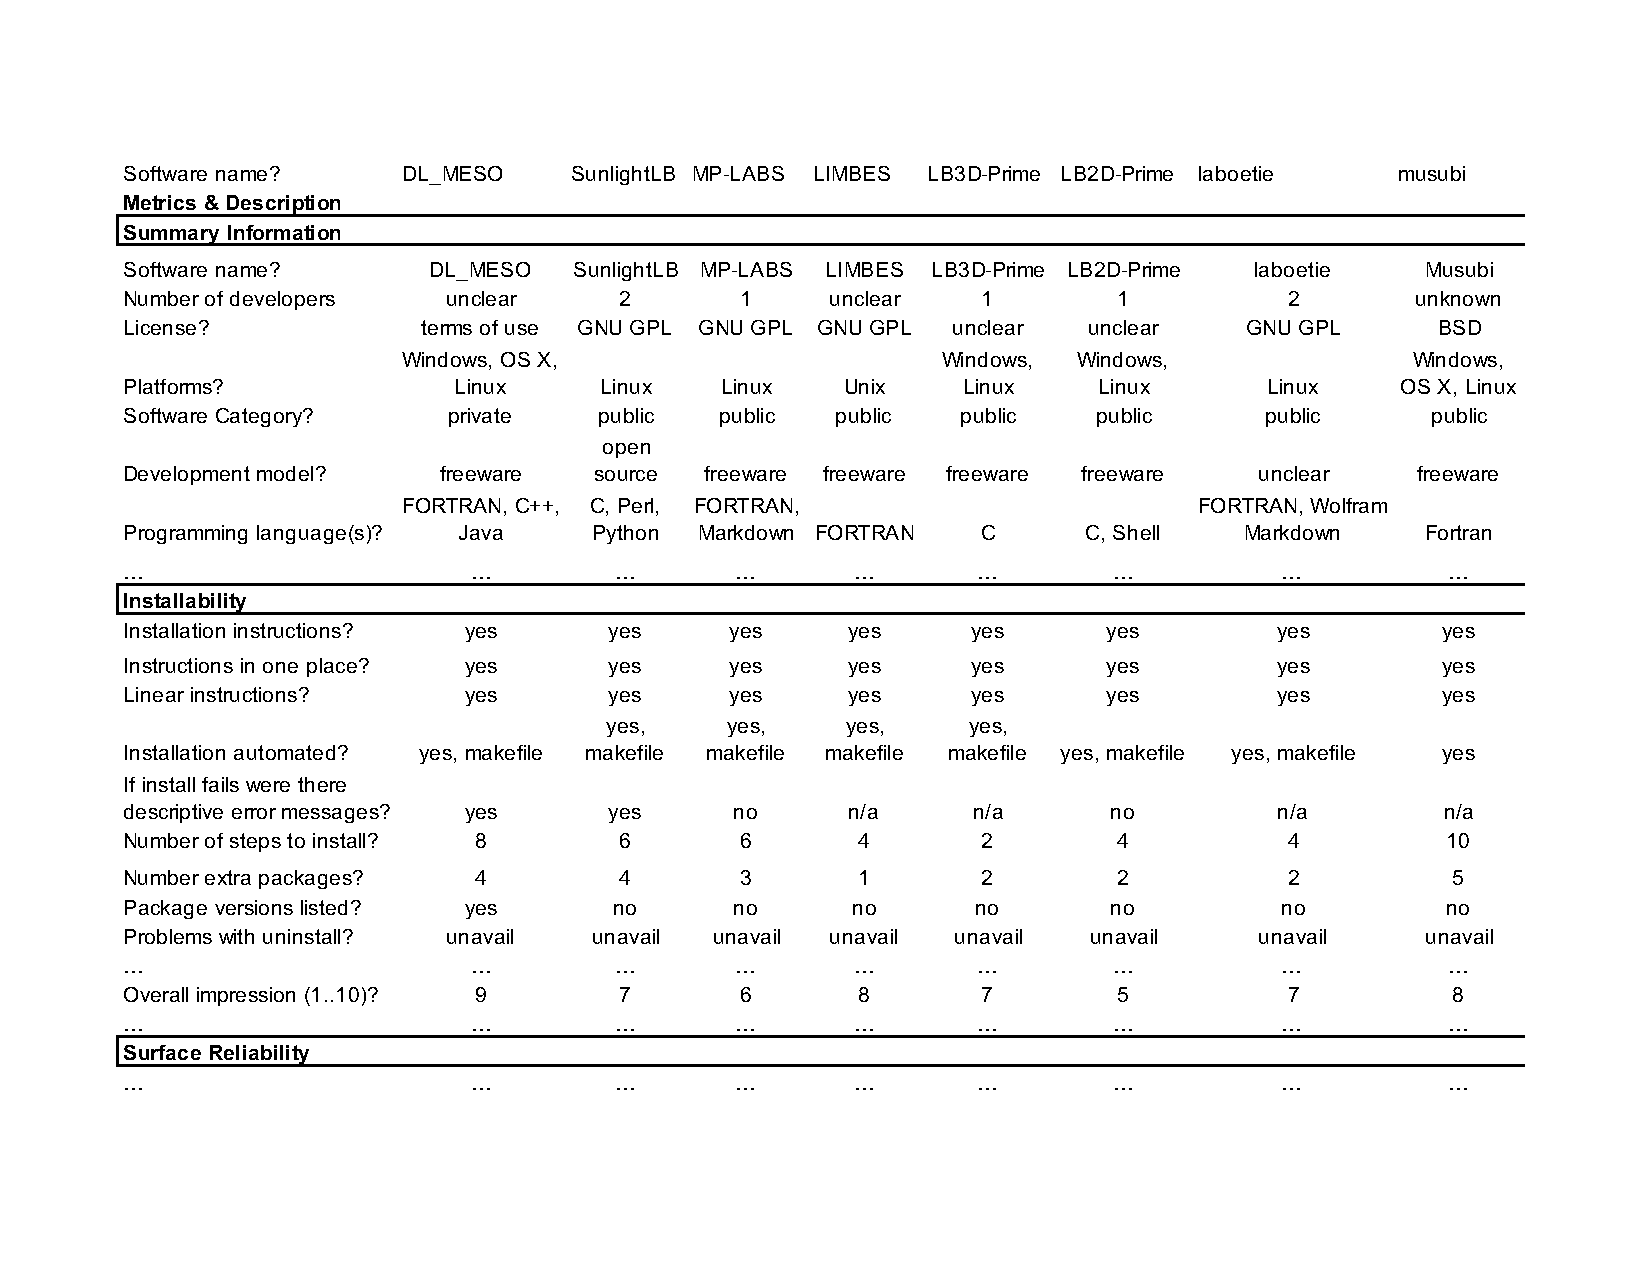
\includegraphics[width=1.0\textwidth]{./figures/measurement_template}
	  \caption{Excerpt of the Top Section of the Measurement Template (Summary
	  Information) \wss{Should update this figure to something easier to read}}
	  \label{measurement_template_image}
	\end{center}
\end{figure}

The full template consists of 108 questions categorized under 9 qualities:
\begin{inparaenum}
	\item installability;
	\item correctness and verifiability;
	\item surface reliability;
	\item surface robustness;
	\item surface usability;
	\item maintainability;
	\item reusability;
	\item surface understandability; and,
	\item visibility/transparency. 
\end{inparaenum} 
The questions were designed to be unambiguous, quantifiable and measurable with
limited time and domain knowledge. The measures are grouped under headings for
each quality, and one for summary information
(Figure~\ref{measurement_template_image}).   The summary section provides
general information, such as the software name, number of developers, etc.  We
follow the definitions given by \citet{GewaltigAndCannon2012} for the software
categories.  Public means software intended for public use.  Private means
software aimed only at a specific group, while the concept category is used for
software written simply to demonstrate algorithms or concepts. The three
categories of development models are: open source, where source code is freely
available under an open source license; free-ware, where a binary or executable
is provided for free; and, commercial, where the user must pay for the software
product.  

Several of the qualities use the word ``surface''.  This is to highlight that,
for these qualities in particular, the best that we can do is a shallow measure
of the quality.  For instance, we are not currently doing any experiments to
measure usability.  Instead, we are looking for an indication that usability was
considered by the developers.  We do this by looking for cues in the
documentation, like a getting started manual, a user manual and documentation of
expected user characteristics.

Most of the data was gathered by manually investigating the software, its source
code, and its artifacts, while some was gathered using the automatic repository
measurement tools.  Tools were use to find data such as the number of files,
number of lines of code (LOC), percentage of issues that are closed, etc. The
tool \href{https://github.com/tomgi/git_stats}{GitStats} was used to measure
each software package's GitHub repository for the number of binary files, the
number of added and deleted lines, and the number of commits over varying time
intervals. The tool \href{https://github.com/boyter/scc}{Sloc Cloc and Code
(scc)} was used to measure the number of text based files as well as the number
of total, code, comment, and blank lines in each GitHub repository.

As in \citet{SmithEtAl2016}, Virtual machines (VMs) were used to provide an
optimal testing environments for each package. VMs were used because it is
easier to start with a fresh environment without having to worry about existing
libraries and conflicts. Moreover, when the tests are complete the VM can be
deleted, without any impact on the host operating system. The most significant
advantage of using VMs is to level the playing field. Every software install
starts from a clean slate, which removes ``works-on-my-computer'' errors. When
filling in the measurement template spreadsheet, the details for each VM
should be noted, including hypervisor and operating system version.

\subsection{Interview Developers} \label{SecSurvey}

We designed a list of 20 questions to guide our interviews, which can be found
in \citet{SmithEtAl2021}. Some questions are about the background of the
software, the development teams, the interviewees, and how they organize the
projects. We also ask about the developer's understandings of the users. Some
questions focus on the current and past difficulties, and the solutions the team
has found, or will try. We also discuss the importance and current situations of
documentation. A few questions are about specific software qualities, such as
maintainability, understandability, usability, and reproducibility. The
interviews are semi-structured based on the question list; we ask follow-up
questions when necessary. Based on our experience, the interviewees usually
bring up some exciting ideas that we did not expect, and it is worth expanding
on these topics.

We requested interviews from all 24 packages, with 4 positive responses.  To
send out interview requests we found we found contacts on the projects’ website,
or code repository, or publications, or the biographic pages of the teams’
institutions. We send at most two interview request emails to a contact for each
software package.  Meeting will typically be held using on-line meeting
software, like Zoom or Teams.  This facilitates recording and automatic
transcription of the meetings.

The interviews followed the standard ethics guideline of asking for consent
before interviewing, recording, and including participant details in the report.
The interview process presented here was approved by the McMaster University
Research Ethics Board under the application number 
\href{https://github.com/smiths/AIMSS/blob/master/StateOfPractice/MACREM/Application.pdf}
{MREB\#: 5219}.

\subsection{Analytical Hierarchy Process} \label{AHP}

The Analytical Hierarchy Process (AHP) is a decision-making technique that is
used to compare multiple options by multiple criteria. In our work AHP was used
for comparing and ranking the LBM software packages using the overall impression
quality scores that were gathered in the measurement template.  AHP performs a
pairwise analysis using a matrix and generates an overall score as well as
individual quality scores for each software package. \citep{SmithEtAl2016} shows
how AHP is applied to ranking software based on quality measures. 

This project used a tool for conducting this process. The tool includes a
sensitivity analysis that was used to ensure that the software package rankings
are appropriate with respect to the uncertainty of the quality scores. For the
sensitivity analysis we modified the score by 10\% for each package and verified
that the overall ranking was stable.  The
\href{https://github.com/smiths/AIMSS/blob/master/StateOfPractice/AHP2020/LBM/README.txt}{README}
file of the tool includes requirements and usage information.

\subsection{Interaction With Domain Expert} \label{sec_vet_software_list}

The Domain Expert is an important member of the state of the practice assessment
team. Pitfalls exist if non-experts attempt to acquire an authoritative list of
software, or try to definitively rank the software. Non-experts have the problem
that they can only rely on information available on-line, which has the
following drawbacks:
\begin{inparaenum}[i)]
  \item the on-line resources could have false or inaccurate information; and,
  \item the on-line resources could leave out relevant information that is so
in-grained with experts that nobody thinks to explicitly record it.
\end{inparaenum}
For the current assessment, our Domain Expert (and paper co-author) is Dr.\
Zahra Motamed, Assistant Professor of Mechanical Engineering at McMaster
University, Hamilton, Ontario, Canada.  

The Domain Expert has an important role with verifying the list of LBM packages.
In advance of the first meeting with the Domain Expert, they were asked to
create a list of top software packages in the domain.  This is done to help the
expert get in the right mind set in advance of the meeting.  Moreover, by doing
the exercise in advance, we avoid the potential pitfall of the expert approving
the discovered list of software without giving it adequate thought.  The Domain
Expert was also asked to vet the collected data and analysis.  In particular,
they were asked to vet the proposed list of software packages and the AHP
ranking.  These interactions were done via virtual meetings.

\section{Quantitative Findings and AHP Results} \label{AHPresults}

Table~\ref{} presents a summary of the software that was measured.  The table
shows the differences between the packages based on features.  \wss{Add some
discussion of some example features.}  The sections below summarize how the
software packages compare based on qualities, as measured by the measurement
template.   The results of the AHP ranking are also discussed.

\begin{table}
	\begin{center}
		\begin{tabular}{ p{3cm}llllllll}
			\hline
			Name & Dim & Pll & Com & Rflx & MFl & Turb & CGE & OS\\
			\hline
			DL\_MESO (LBE) & 2, 3 & Y & Y & Y & Y & Y & Y & W, M, L\\
			ESPResSo & 1, 2, 3 & Y & Y & Y & Y & Y & Y & M, L\\
			ESPResSo++ & 1, 2, 3 & Y & Y & Y & Y & Y & Y & L\\
			HemeLB & 3 & Y & Y & Y & Y & Y & Y & L\\
			laboetie & 2, 3 & Y & Y & Y & Y & Y & Y & L\\
			LatBo.jl & 2, 3 & N & Y & Y & Y & N & Y & L\\
			LB2D-Prime & 2 & Y & Y & Y & Y & Y & Y & W, L\\
			LB3D & 3 & Y & N & Y & Y & Y & Y & L\\
			LB3D-Prime & 3 & Y & Y & Y & Y & Y & Y & W, L\\
			lbmpy & 2, 3 & Y & Y & Y & Y & Y & Y & L\\
			lettuce & 2, 3 & N & Y & Y & Y & Y & Y & W, M, L\\
			LIMBES & 2 & Y & Y & Y & N & N & Y & L\\
			Ludwig & 2, 3 & Y & Y & Y & Y & Y & Y & L\\
			LUMA & 2, 3 & Y & Y & Y & Y & Y & Y & W, M, L\\
			MechSys & 2, 3 & N & Y & Y & Y & Y & Y & L\\
			MP-LABS & 2, 3 & Y & N & Y & Y & N & N & L\\
			OpenLB & 1, 2, 3 & Y & Y & Y & Y & Y & Y & W, M, L\\
			Palabos & 2, 3 & Y & Y & Y & Y & Y & Y & W, L\\
			pyLBM & 1, 2, 3 & Y & Y & Y & N & Y & Y & W, M, L\\
			Sailfish & 2, 3 & Y & Y & Y & Y & Y & Y & M, L\\
			SunlightLB & 3 & N & Y & Y & N & N & Y & L\\
			TCLB & 2, 3 & Y & Y & Y & Y & Y & Y & L\\
			waLBerla & 2, 3 & Y & Y & Y & Y & Y & Y & L\\
			\hline
		\end{tabular}
		\caption{Features of Software Packages (Dim for Dimension (1, 2, 3),
			Pll for Parallel (Yes or No), Com for Compressible (Yes or No), Rflx for
			Reflexive Boundary Condition (Yes or No), MFl for Multifluid (Yes or
			No), Turb for Turbulent (Yes or No), CGE for Complex Geometries (Yes or No), OS for Operating System (Windows (W), macOS (M), Linux (L)))} \label{tbl_features}
	\end{center}
\end{table}

\subsection{Installability}

All of the 23 software packages that were tested have installation instructions.
As noted previously, many of the 23 software packages that were part of the
original long list of 45 packages were removed due to not including
documentation or installation instructions. Of the 23 software packages that
were tested, most had installation instructions located in one place, often in
an instruction manual or on a web-page. Sometimes, like with Ludwig, incomplete
installation instructions are found on a home page, with more detailed
instructions located on another web-page, or within the documentation.
Maintainability and correctness of these instructions could be improved if all
the instructions were in one location. 

All 23 packages on the short list can be installed on some Unix-like systems.
Seven packages could be installed on Windows, and five on macOS. Operating
system compatibility is found in the documentation of 19 software packages. All
but one of the software packages (TCLB) were tested on Ubuntu for this state of
the practice assessment. TCLB was tested on CentOS, since this operating system
is mentioned in its installation instructions.

All but one of the software packages (LatBo.jl) have automated at least some of
the installation process. Most of these packages, such as waLBerla and
SunlightLB, use Make to automate the installation, and a few of them, like
lbmpy, use custom scripts.

Errors encountered during the installation process were often quickly fixed
thanks to descriptive error messages. Systems that provided vague error
messages, such as messages that did not specify which action or file was at
fault, were more difficult to troubleshoot. Only three software packages
(HemeLB, LB3D, lbmpy) that displayed a descriptive error message were not
recoverable, and most of these instances were due to hardware and operating
system incompatibility, such as the requirement of CUDA. Fourteen software
packages definitively broke during installation. Some packages, such as
LB2D-Prime and LB3D-Prime, did not provide a definitive message of the success
or failure of installation. In these instances, validating the installation
required performing a tutorial or running a script, as described below, if these
were available. 

About half of the installation instructions are written as if the person doing
the installation has none of the dependent packages installed. Unfortunately,
software packages, like ESPResSo++, Ludwig, and LUMA, frequently don't list all
of their dependencies, or provide only a partial list. Sometimes only an error
message during the installation process informs the user of the requirement of
these additional packages. A detailed rewrite of the installation instructions
from the point of view of installation on a clean operating system is suggested.
A clean environment can be achieved for testing purposes by using a virtual
machine.

Sixteen software packages require less than 10 dependencies to be installed. All
but one software package (LatBo.jl) require less than 20 dependencies. Some
packages may automatically install additional dependencies in the background.
Eighteen of the software packages do not explicitly indicate software dependency
versions. Some software package installation issues, specifically those
occurring when manual installation of dependencies is required, may be avoided
if versions of dependencies are specified. Fifteen software packages do not have
detailed instructions for installing dependencies. Sixteen software packages
have less than 10 manual installation steps. If dependencies are installed in
one command then none of the software packages take more than 20 steps to
install. The average number of steps is about eight, and the fewest is two
(LB3D-Prime). 

All but six (ESPResSo, HemeLB, laboetie, LB3D-Prime, lbmpy, waLBerla) of the
software packages have a way to verify the installation. Most have some sort of
tutorial examples that can be run by the user. Some other ways of installation
validation include validation scripts (LB2D-Prime, lettuce, Ludwig, LUMA),
automatic validation after the installation (LatBo.jl), and instructions to
manually review the file system (LIMBES).  Uninstallation instructions were
found for only one of the software packages: pyLBM.

\begin{figure}[h!]
	\begin{center}
		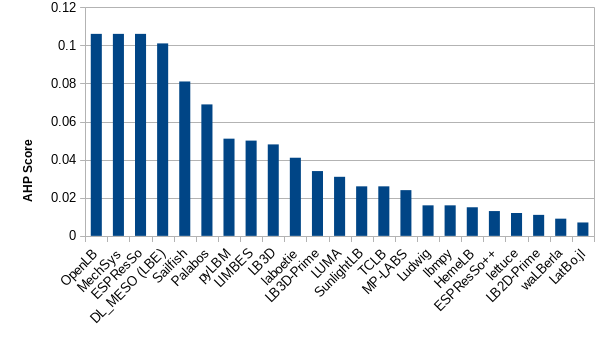
\includegraphics[width=1.0\textwidth]{./figures/installability_chart}
		\caption{AHP Installability Score}
		\label{Fig_Installability}
	\end{center}
\end{figure}

Figure~\ref{Fig_Installability} shows the installability ranking of the software
packages using AHP. Software packages with a higher score (MechSys, Palabos,
ESPResSo, OpenLB) tend to have one set of linear installation instructions that
are written as if the person doing the installation has none of the dependencies
installed. The instructions often list compatible operating system versions and
include instructions for the installation of dependencies. The top ranked
packages often incorporate some sort of automation of the installation process
and have fewer manual installation steps. The number of dependencies a package
has does not correlate with a higher score. The ability to validate the
installation process, often through tutorials or test examples that include
expected output, is correlated with a higher score. Furthermore, the top six
ranked packages are noted as being alive. 

Many software packages would benefit from a rewrite or reorganization of
installation instructions. A single location for installation instructions would
improve their maintainability and correctness. Listing compatible operating
system and dependency versions would decrease installation time and errors, as
would adding instructions on installing dependencies. Installation process
errors should prompt the system to display detailed messages. Once a software
package is installed, either an automatic validation needs to be performed or
the user needs to be able to perform a manual validation using test examples
that include expected output. Finally, uninstallation instructions should be
included in the documentation. 
 
\subsection{Surface Correctness and Verifiability}

Sixteen of the software packages include a requirements specification artifact
or explicitly reference domain theory, often only the latter. Software packages
that distribute requirements specification information, such as DL\_MESO (LBE),
generally keep it brief and include it within other documentation. This artifact
is often found within a user manual, on a web-page, or is mentioned in related
publications. In the latter case the user may need to spend significant time to
find this information. 

Document generation tools are explicitly used by 12 software packages. Sphinx is
used by eight of them, and Doxygen is used by seven. Several of the packages use
both.

Tutorials are available for 18 of the software packages. Generally they are
linearly written and easy to follow. However, only eight tutorials provide an
expected output. It is not possible to verify the correctness of the output of
the software packages that are missing this key information. In these cases the
user may need to assume correctness if there are no visible errors.

Unit tests are only explicitly available for one of the software packages,
Ludwig. Code modularization of most packages allow for users to create tests
with varying degrees of effort. These tests allow developers and users to verify
the correctness of fragments of the source code, and in doing so better assess
the correctness of the entire package.

The use of continuous integration tools and techniques alludes to a more refined
development process where faults are isolated and better recognized. Only two of
the packages (ESPResSo, Ludwig) mentioned applying the practice of continuous
integration in their development process. 

\begin{figure}[h!]
	\begin{center}
		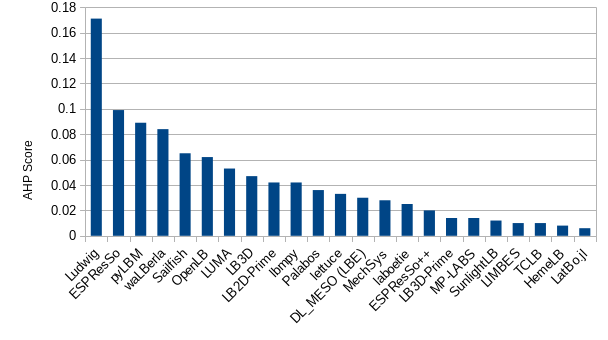
\includegraphics[width=1.0\textwidth]{./figures/correctnessverifiability_chart}
		\caption{AHP Surface Correctness and Verifiability Score}
		\label{Fig_CorrectnessVerifiability}
	\end{center}
\end{figure}

Figure~\ref{Fig_CorrectnessVerifiability} shows the surface correctness and
verifiability ranking of the software packages using AHP. Software packages with
a higher score tend to have a visible requirements specification or references
to theory documentation. They also explicitly use at least one document
generation tool that builds confidence of correctness. The top ranked software
packages all include an easy to follow getting started tutorial, and most of
these include expected output. Only the top ranked package, Ludwig, provided
unit testing. It and the second ranked package, ESPResSo, explicitly
incorporated continuous integration in the development process. Furthermore,
eight of the top 10 ranked packages are noted as being alive.

The inclusion of requirements specification and theory documentation greatly
benefits the correctness and verifiability of software packages. The use of
document generation tools can help build confidence in correctness. The addition
of easy to follow tutorials further helps users verify the software and have
confidence in its correctness. Unit testing, as well as the use of continuous
integration tools and techniques such as Bamboo, Jenkins, and Travis CI, help
verify correctness.

\subsection{Surface Reliability}

The analysis of surface reliability focused on package installation and
tutorials. Errors occurred when installing 16 of the software packages. Every
instance prompted an error message. These messages indicated unrecognized
commands (even when following the installation guide), missing links, missing
dependencies, and syntax errors in code files. In some instances the error messages
were vague. Several automatic installation processes could not find and load
dependencies. In these instances the installation tried to access outdated
external repositories. Seven of the installations were recovered and verified,
and one of the installations (LB3D-Prime) was assumed to be recovered due to the
absence of any way to verify it. The installation of eight of the software
packages could not be recovered. Most of these broken installations could not
find external dependencies, encountered system incompatibilities, or displayed
vague error messages. 

Of the 13 software packages that installed correctly and also have tutorials,
four (pyLBM, ESPResSo++, LIMBES, Ludwig) broke during tutorial testing. All of
these instances resulted in an error message being displayed. One error (pyLBM)
was due to a missing tutorial dependency, another (Ludwig) was due to an invalid
command despite following the tutorial, and the final two errors were vague
execution errors. Of the four broken tutorial instances, only the one that was
missing a dependency was recoverable. 

\begin{figure}[h!]
	\begin{center}
		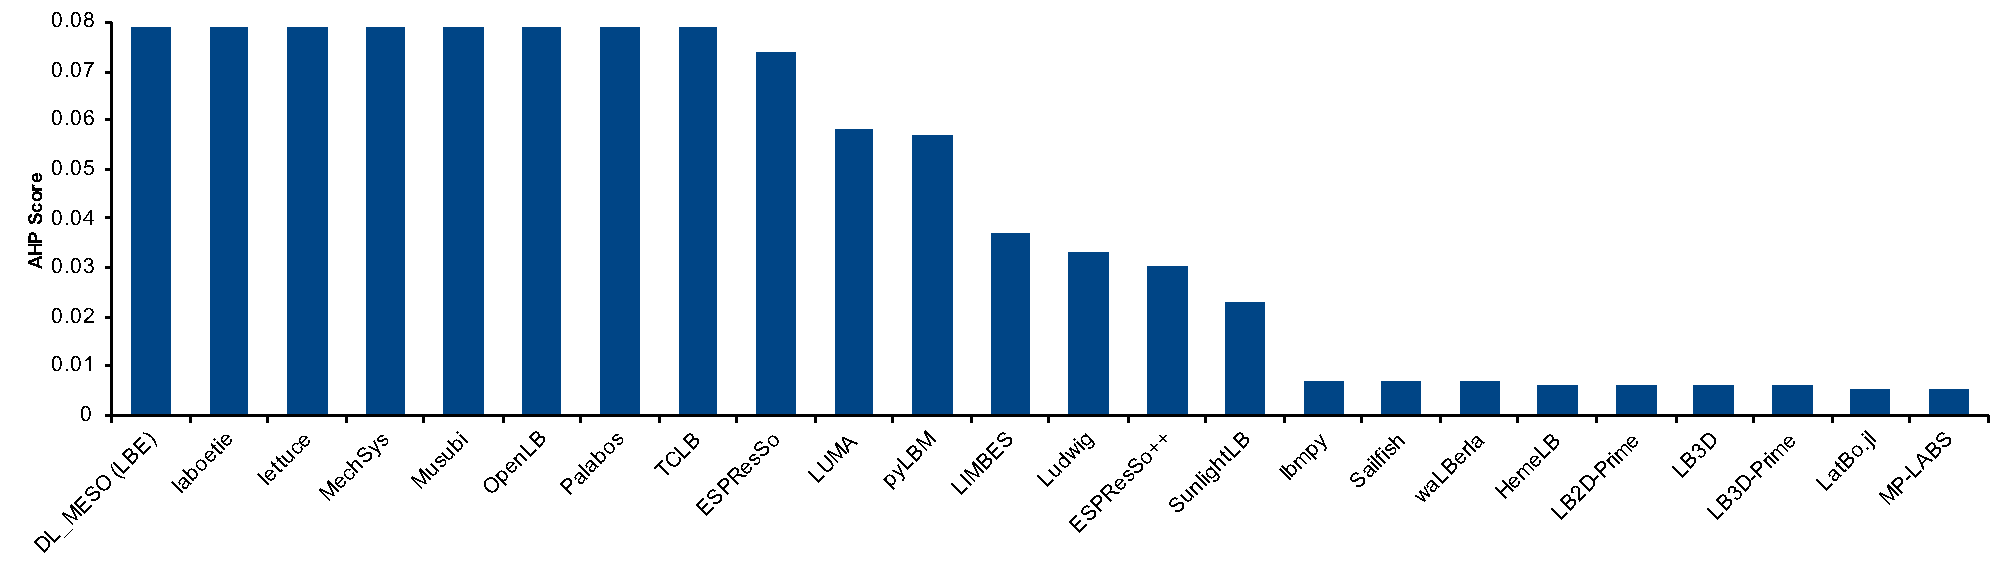
\includegraphics[width=1.0\textwidth]{./figures/reliability_chart}
		\caption{AHP Surface Reliability Score}
		\label{Fig_Reliability}
	\end{center}
\end{figure}

Figure~\ref{Fig_Reliability} shows the surface reliability ranking of the
software packages using AHP. Software packages with a high score either did not
break during installation, or the broken installation was recoverable. All of
the top five ranked packages have tutorials. One of these packages, pyLBM, broke
during tutorial testing, but a descriptive error message helped in recovery.
Furthermore, nine of the top 10 ranked packages are noted as being alive. 

Overall, lower ranked software packages are lacking clear documentation, testing
or tutorial examples, and descriptive error messages, and have broken
dependencies. Thus, regarding surface reliability, software packages would
benefit from clear up-to-date documentation that specifies all dependencies, the
inclusion of testing and tutorial examples, and the assurance of descriptive
error messages after faults.

\subsection{Surface Robustness}

The software packages were tested for handling unexpected input, including
incorrect data types, empty input, and missing files or links. Success
predicated on a reasonable response from the system, including appropriate error
messages and an absence of unrecoverable system failures. 

\begin{figure}[h!]
	\begin{center}
		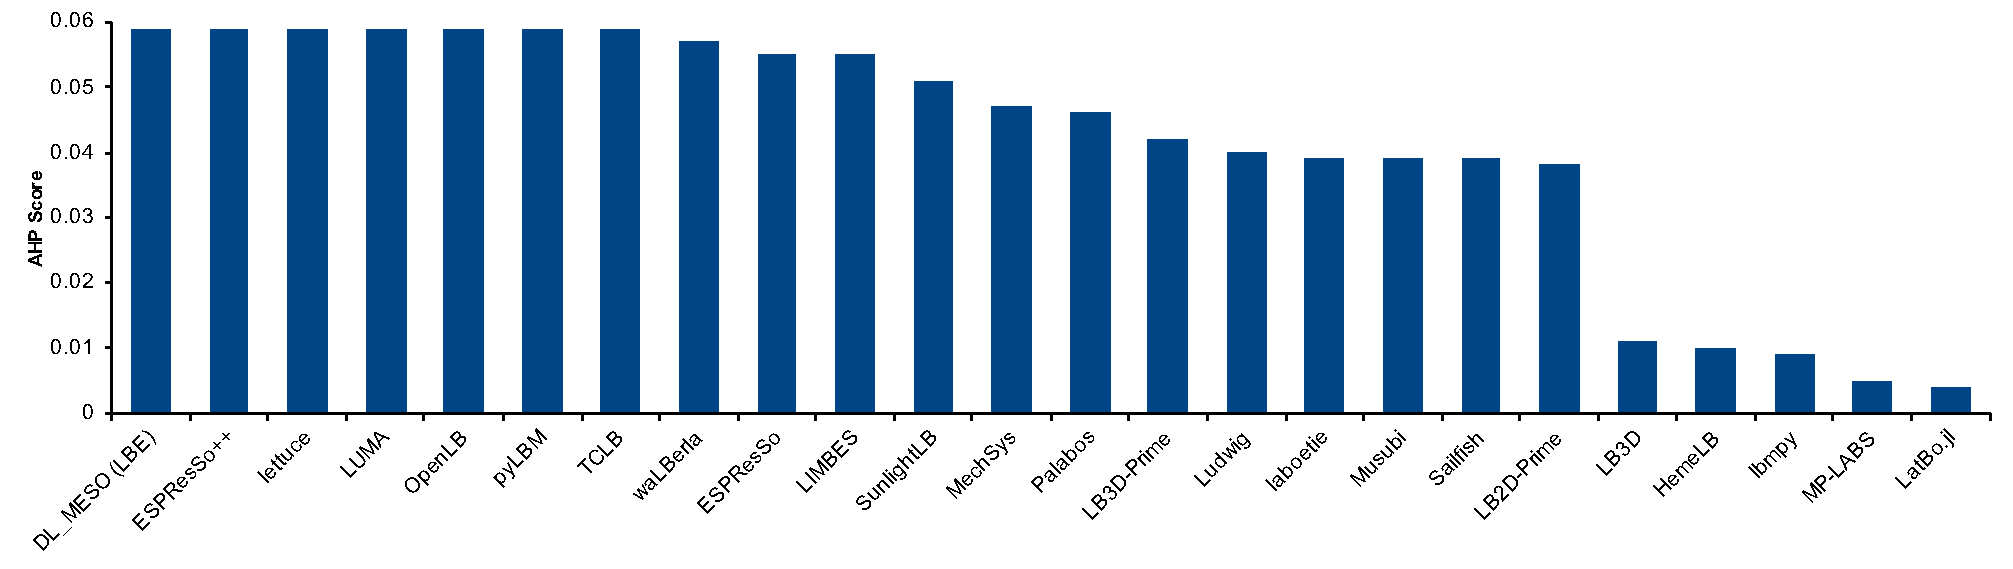
\includegraphics[width=1.0\textwidth]{./figures/robustness_chart}
		\caption{AHP Surface Robustness Score}
		\label{Fig_Robustness}
	\end{center}
\end{figure}

Figure~\ref{Fig_Robustness} shows the surface robustness ranking of the software
packages using AHP. Software packages with a high score behaved reasonably in
response to unexpected input as described above. All of the software packages
that installed correctly passed this test. They output descriptive error
messages or did not crash. Software packages with a lower surface robustness
score did not install correctly, so their robustness score may not be a true
reflection of runtime robustness. All successfully installed software packages
that require a plain text input file correctly handled an unexpected change to
these input files, including a replacement of new lines with carriage returns.
Furthermore, nine of the top 10 ranked packages are noted as being alive. LIMBES
is noted as being classified as dead.

\subsection{Surface Performance}

Although the software packages all apply LBM to solve scientific computing
problems, the packages focus on varied CFD problems, with varying parameters,
and are technically different from each other (as shown in
Table~\ref{tbl_features}). Due to this, a comparison of performance is not
appropriate. In this project we instead looked through each software package's
artifacts for evidence that performance was considered. The artifacts of 17
software packages mentioned parallelization. This included GPU processing and
the CUDA parallel computing platform, which were mentioned in the artifacts of 6
packages (ESPResSo, lbmpy, lettuce, pyLBM, Sailfish, TCLB). GPUs provide
superior processing power and speed compared to CPUs, and are often used for
scientific computing when a large amount of data is involved. The software
package TCLB is implemented in a highly efficient multi-GPU code to achieve
performance suitable for model optimization \citep{rutkowski2020open}. In the
Ludwig package, a so-called mixed mode approach is used where fine-grained
parallelism is implemented on the GPU, and MPI is used for even larger scale
parallelism \citep{gray2013ludwig}. While one software package (Sailfish)
required CUDA and GPU processing, some (ESPResSo, lbmpy, lettuce, pyLBM, TCLB)
have the option of using either the GPU or the CPU. The packages that require
GPU and CUDA have better performance at the expense of installability and
surface reliability.

\subsection{Surface Usability}

Software package artifacts were reviewed for the presence of a tutorial, a user
manual, documented user characteristics, and a user support model. In total 18
software packages have a tutorial, 13 have a user manual, and 11 have both. The
tutorials vary in scope and substance, and eight include expected output.
Most user manuals are in the form of a file that can be downloaded, while some
are rendered on a web-page. Some packages (waLBerla) do not have a user manual,
but do have useful documentation distributed on their web-pages. Expected user
characteristics are documented in four software packages (laboetie, LIMBES,
Ludwig, Palabos). Users are typically scientists or engineers. Their background
is often physics, chemistry, biophysics, or mathematics. All but one of the
packages (LIMBES) have a user support model, and many of them have multiple
avenues of user support. The most popular avenue of support is Git, followed by
email and forums. One software package (OpenLB) has an FAQ page.    

\begin{figure}[h!]
	\begin{center}
		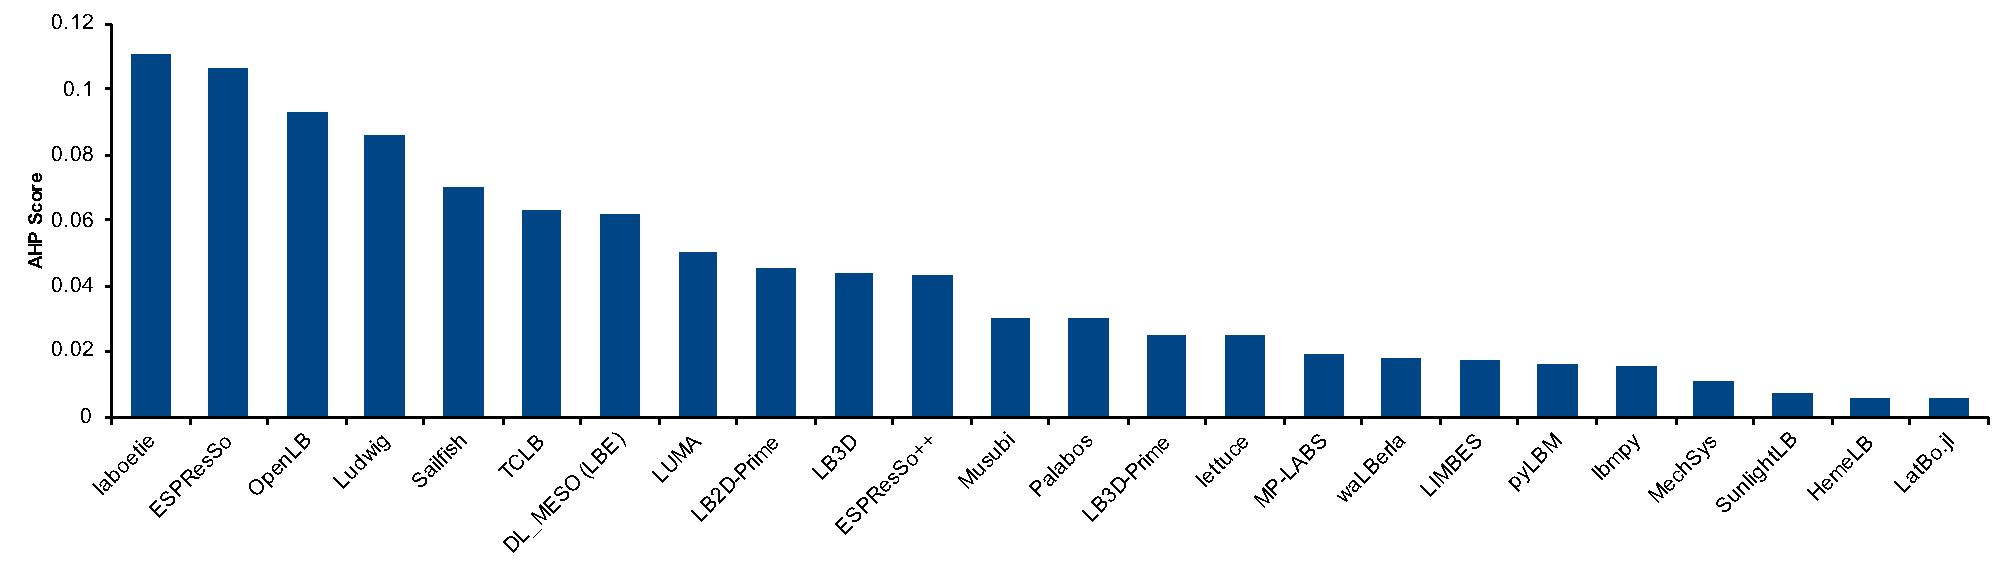
\includegraphics[width=1.0\textwidth]{./figures/usability_chart}
		\caption{AHP Surface Usability Score}
		\label{Fig_Usability}
	\end{center}
\end{figure}

Figure~\ref{Fig_Usability} shows the surface usability ranking of the software
packages using AHP. Software packages with a high score have a tutorial and user
manual, sometimes have documented user characteristics, and have at least one
user support model. Many packages have several user support models. Furthermore,
four of the top five ranked packages are noted as being alive. 

\subsection{Maintainability}

Software packages were reviewed for the presence of artifacts. Every type of
artifact or file that is not a code file was recorded. The software packages
were also reviewed for software release and documentation version numbers. This
information can be used to troubleshoot issues and organize documentation. All
but three software packages (LatBo.jl, LB3D-Prime, MechSys) have source code
release and documentation version numbers.

When present, information on how code is reviewed, or how to contribute to the
project was also noted. In total, 11 software packages have this information,
which was found in various artifacts, including in developer guides, contributor
guides, user guides, developer web-pages, and README files. 

Issue tracking is used in 22 software packages, 15 of which use Git, six use
email, and one (SunlightLB) uses SourceForge. Most software packages that use
Git have most of their issues closed, and only three (laboetie, lettuce,
Sailfish) have less than 50 percent of their issues closed. Four of the top five
overall ranked packages (Ludwig, ESPResSo, Palabos, LUMA) have most of their
issues closed. Fourth ranked LUMA does not use Git. Alive packages (11 use Git
issue tracking) have 64\% of their issues closed, while dead packages (3 use Git
issue tracking) have 71\% of their issues closed. This information is presented
in Table~\ref{gitrepodata}. Furthermore, 13 packages that use Git for issue
tracking use GitHub as a version control system, while two (Palabos, waLBerla)
use GitLab. Of the other packages, one package (SunlightLB) uses CVS for issue
tracking, and seven packages do not appear to use any issue tracking system.

\begin{table}
	\begin{center}
		\begin{tabular}{ p{3.5cm}p{3.5cm}p{3.5cm}p{2.5cm} }
			\hline
			Name & $\%$ Issues Closed & $\%$ Code Comments & Status\\
			\hline
			DL\_MESO (LBE) & Not Git & 8.06& Alive\\
			ESPResSo & 89.26 & 21.78 & Alive\\
			ESPResSo++ & 66.28 & 17.10 & Alive\\
			HemeLB & No Issues & 16.68 & Dead\\
			laboetie & 18.75 & 2.47 & Dead\\		
			LatBo.jl & 93.33 & 0.40 & Dead\\
			LB2D-Prime & Not Git & 13.61 & Dead\\
			LB3D & Not Git & 13.76 & Dead\\
			LB3D-Prime & Not Git & 14.34 & Dead\\
			lbmpy& 58.33  & 2.03 & Alive\\
			lettuce & 33.33 & 8.19 & Alive\\
			LIMBES & Not Git & 17.39 & Dead\\
			Ludwig& 60.00 & 20.70 & Alive\\
			LUMA& 85.71   & 0.20 & Alive\\
			MechSys & Not Git & 15.11 & Alive\\
			MP-LABS & 100.00 & 26.67 & Dead\\
			OpenLB & Not Git & 22.43 & Alive\\
			Palabos & 89.47 & 17.76 & Alive\\
			pyLBM & 66.67& 16.12 & Alive\\
			Sailfish & 22.22 & 9.26 & Alive\\
			SunlightLB & Not Git & 17.67 & Dead\\
			TCLB & 60.32 & 6.02 & Alive\\
			waLBerla & 72.90 & 22.62 & Alive\\
			\hline
		\end{tabular}
		\caption{Git Repository Data} \label{gitrepodata}
	\end{center}
	\end{table}
		
Software package code files were further measured for the percentage of code
that is comments. The findings are presented in Table~\ref{gitrepodata}.
Packages with a higher percentage of comments were designated as more
maintainable. Comments represent more than 10 percent of code files in 15
packages, and the average percentage of code comments is about 14 percent. Four
of the top five overall ranked packages (Ludwig, ESPResSo, Palabos, OpenLB) have
more than the average. Fifth ranked LUMA has only 0.2 percent comments, the
fewest of any package. This package has the most lines of source code, with over
four million. The next largest package is ESPResSo++ with one million.

\begin{figure}[h!]
	\begin{center}
		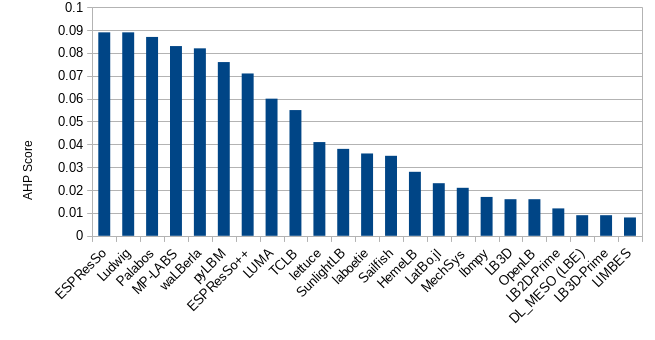
\includegraphics[width=1.0\textwidth]{./figures/maintainability_chart}
		\caption{AHP Maintainability Score}
		\label{Fig_Maintainability}
	\end{center}
\end{figure}

Figure~\ref{Fig_Maintainability} shows the maintainability ranking of the
software packages using AHP. Software packages with a high score provide version
numbers on documents and source code releases, have an abundance of high quality
artifacts, and use an issue tracking tool and version control system. These
packages also appear to reasonably handle issue tracking, having most of their
issues closed. Their code files are well commented with more than 10 percent of
the code being comments. Furthermore, nine of the top 10 ranked packages are
noted as being alive. MP-LABS is noted as being dead.\\

\wss{Sort ``Git Repository Data'' table in descending order of percentage of
code comments.}

\subsection{Reusability} \label{reusabilityresults}

We measured the total number of source code files for each project. A larger
number of source files is associated with increased reusability, due to our
assumption that this indicates increased modularization. Some packages have more
features than others.  This is assumed to contribute to reusablility, since they have
more source code for potential reuse. The software packages were also reviewed
for the presence of API documentation, which indicates that a software package
was developed with interaction between other software applications in mind. 

\begin{figure}[h!]
	\begin{center}
		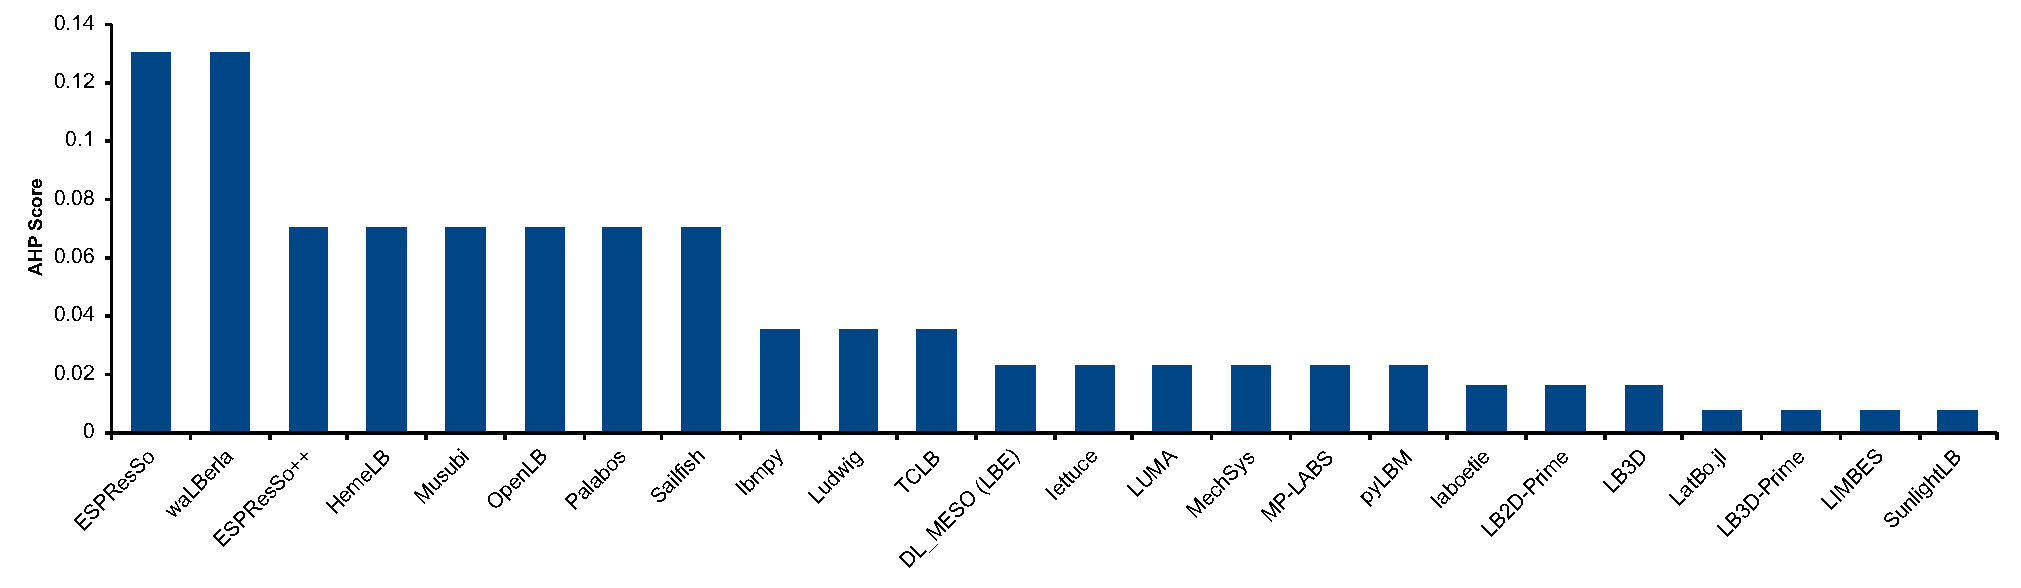
\includegraphics[width=1.0\textwidth]{./figures/reusability_chart}
		\caption{AHP Reusability Score}
		\label{Fig_Reusabilty}
	\end{center}
\end{figure}

Figure~\ref{Fig_Reusabilty} shows the reusability ranking of the software
packages using AHP. Software packages with a high score have thousands of source
code files and API documentation. The highest scoring packages, ESPResSo and
waLBerla, have extensive functionality, including graphical visualizations and
non-LBM modeling. For this reason, a comparison with other software packages is
not on a level field. However, these packages do have an abundance of reusable
components. Furthermore, nine of the top 10 ranked packages are noted as being
alive. HemeLB is considered to be dead.

\begin{table}
	\begin{center}
		\begin{tabular}{ p{3.5cm}p{2cm}p{2.5cm}p{2cm}p{2.5cm} }
			\hline
			Name & Text Files & Binary Files & LOC & Avg. LOC / Text File\\
			\hline
			DL\_MESO (LBE) & 310 & 51 & 170223 & 549\\
			ESPResSo & 1309& 86 & 186700 & 143\\
			ESPResSo++ & 5328& 66 & 969196 & 182\\
			HemeLB & 1065& 48 & 95104 & 89\\
			laboetie & 133& 1 & 48403 & 364\\		
			LatBo.jl & 41& 0 & 42172 & 1029\\
			LB2D-Prime & 82& 19 & 54755 & 668\\
			LB3D & 99 & 76 & 39766 & 402\\
			LB3D-Prime & 2 3& 6 & 12944 & 563\\
			lbmpy& 201 & 28 & 46489 & 231\\
			lettuce & 62 & 0 & 5529 & 89\\
			LIMBES & 26 & 1 & 4872 & 187\\
			Ludwig & 859 & 32 & 109811 & 128\\
			LUMA & 312 & 19 & 4370670 & 14000\\
			MechSys & 324 & 3 & 85543 & 264\\
			MP-LABS & 307 & 3 & 43124 & 140\\
			OpenLB & 1104 & 5 & 209034 & 189\\
			Palabos & 1829 & 67 & 547623 & 299\\
			pyLBM & 258 & 85 & 32314 & 125\\
			Sailfish & 632 & 11 & 69398 & 110\\
			SunlightLB & 36 & 1 & 7646 & 212\\
			TCLB & 535 & 7 & 43226 & 81\\
			waLBerla & 2395 & 67 & 848146 & 353\\
			\hline
		\end{tabular}
		\caption{Module Data} \label{moduledata}
	\end{center}
\end{table}

Table~\ref{moduledata} shows file and Lines Of Code (LOC) data for the software
packages. Packages with a high reusability score do not have as many LOC per
text file, generally having a few hundred lines or less. This suggests that the
source code of these packages is likely functionally modularized, and modules
could be reused in other projects.

There was a strong focus on modularity when designing the waLBerla framework to
enhance productivity, reusability, and maintainability
\citep{bauer2021walberla}. The design of waLBerla has enabled it to be
successfully applied in several projects as a basis for various extensions
\citep{bauer2021walberla}.

\subsection{Surface Understandability}

Ten random source code files of each software package were reviewed for several
measures. This assessment of surface understandability may not perfectly reflect
each package, due to the practical limitation of only examining 10 files. 

All of the packages appear to have consistent indentation and formatting. Only
LUMA and HemeLB explicitly identify coding standards that are used during
development. Generally, the software packages use consistent, distinctive, and
meaningful code identifiers. Only four packages (LB2D-Prime, LB3D-Prime, LIMBES,
MP-LABS) appear to use vague identifiers, such as single letters for variables.
Symbolic constants were observed in the source code of 12 packages. The
constants are used for various parameters, mathematical constants, and matrix
definitions. All of the packages are reasonably well commented, with the
comments clearly indicating what is being done (as opposed to how it is being
done). Domain algorithms are noted in the source code of 11 packages.
Table~\ref{moduledata} suggests that the software packages are modularized to
various degrees. When observing the source code files, it was found that 13 of
the packages have a consistent style and order of function parameters.

\begin{figure}[h!]
	\begin{center}
		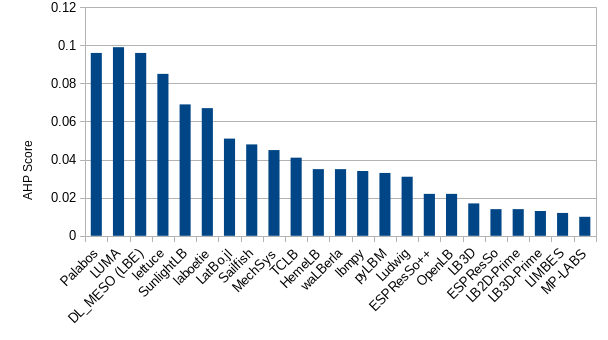
\includegraphics[width=1.0\textwidth]{./figures/understandability_chart}
		\caption{AHP Understandability Score}
		\label{Fig_Understandability}
	\end{center}
\end{figure}

Figure~\ref{Fig_Understandability} shows the surface understandability ranking
of the software packages using AHP. Software packages with a high score have a
consistent indentation and formatting style, and consistent, distinctive, and
meaningful code identifiers. They also have symbolic constants, and explicitly
identify mathematical and LBM algorithms. Their comments are clear and indicate
what is being done in the source code. The source code is well modularized and
structured. Furthermore, four of the top five ranked packages are noted as being
alive.

\subsection{Visibility and Transparency}

Software package artifacts were reviewed for the identification of a specific
development model, like a waterfall of agile development model, and the presence
of documentation recording the development process and standard. They were also
reviewed for the identification of the development environment, and the presence
of release notes. The packages tended to not explicitly use well-known
development models. This was also noted in the interviews with developers, as
detailed below. The development teams of these packages are fairly small and
easily organized without the need for such processes. Seven of the software
packages did have some artifacts outlining the general development process, how
to contribute, and the status of the package or its components. Eight of the
packages have artifacts that note the development environment. While this
information could help developers, and would improve transparency, the small
close-knit nature of the development teams make explicitly publicly specifying
this information practically unnecessary. Version release notes were found in
nine of the software packages.

\begin{figure}[h!]
	\begin{center}
		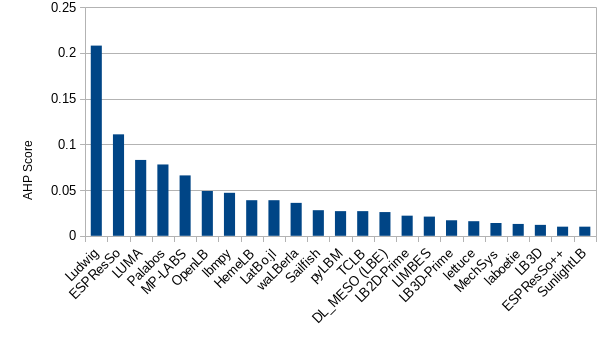
\includegraphics[width=1.0\textwidth]{./figures/visibilitytransparency_chart}
		\caption{AHP Visibility and Transparency Score}
		\label{Fig_VisibilityTransparency}
	\end{center}
\end{figure}

Figure~\ref{Fig_VisibilityTransparency} shows the visibility and transparency
ranking of the software packages using AHP. Software packages with a high score
have an explicit development model and defined development process. They also
had detailed and easy to access notes accompanying software releases.
Furthermore, four of the top five ranked packages are noted as being alive.
MP-LABS is noted as being dead.

\subsection{Overall Quality}

\begin{figure}[h!]
	\centering
		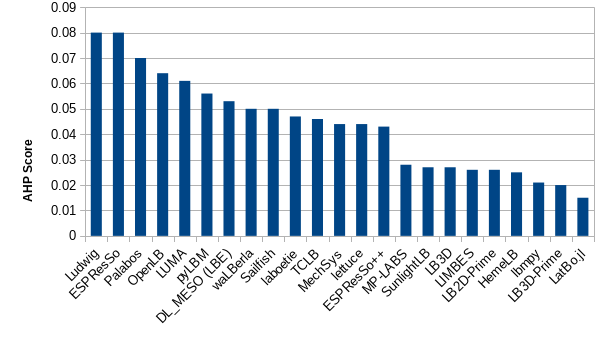
\includegraphics[width=1.0\textwidth]{./figures/finalscore_chart}
		\caption{AHP Overall Score}
		\label{Fig_OverallScore}
\end{figure}

Figure~\ref{Fig_OverallScore} shows the overall ranking of the software packages
using AHP. In the absence of other information on priorities, the overall
ranking was calculated by assuming an equal weighting between all qualities. If the
qualities were weighed differently, the overall software package ranking would
change. Software packages with an overall high score ranked high in at least
several of the individual qualities that were quantitatively measured. 

Looking at the top three ranked packages: Ludwig scored high in surface
correctness and verifiability, surface robustness, surface usability,
maintainability, and visibility and transparency. ESPResSo had achieved a
relative high score in installability, surface correctness and verifiability,
surface usability, maintainability, reusability, and visibility and
transparency. Palabos scored high in installability, surface reliability,
surface robustness, maintainability, and understandability. 

\section{Qualitative Findings From Developer Interviews} \label{interviewresults}

The interview process
presented here was approved by the McMaster University Research Ethics Board
under the application number 
\href{https://github.com/smiths/AIMSS/blob/master/StateOfPractice/MACREM/Application.pdf}
{MREB\#: 5219}.

This section presents the qualitative findings from data that was gathered
during interviews with developers for qualities listed in Section
~\ref{softwarequalities}. The interview questions are found in Appendix
~\ref{interviewquestions}.

\subsection{Surface Correctness and Verifiability}

Interviews with developers confirmed that these software packages are developed
by domain experts with backgrounds in physics, mathematics and mechanical
engineering. It was noted in these interviews that some of the developers do not
have formal software engineering education. Some of the development teams
include computer scientists. Despite a lack of visible domain documentation and
a resulting lower surface correctness and verifiability score, it is clear that
some of the software packages were developed by teams with significant domain
knowledge on account of the academic backgrounds of their developers. 

Interviews suggested a more frequent use of both unit testing and continuous
integration in the development processes than what was observed from the initial
survey. For example, OpenLB, pyLBM, and TCLB use such methods during development
despite this not being explicitly clear from an analysis of the material
available online. The correctness and verifiability of such packages is not
measured well using surface analysis.

Several interviewed developers alluded to difficulty with testing the
correctness of large numbers of features, and some even manually tested program
output. The use of well defined unit testing tools could decrease the time spent
testing some feature.

\subsection{Surface Usability}

Interviews with developers revealed several usability issues. Some users have
misunderstood the boundaries of LBM and CFD, and have combined or applied
methods that are not physically sound. Sometimes users have applied LBM to
poorly defined or inappropriate fluid dynamics problems. For example, they may
wish to model flow through or around a structure despite having limited
information about the structure or its environment, and having little previous
knowledge of CFD. The users do not realize the limitations of the methods, of
the software, and do not understand the requirements to properly model a problem
with the software. As the developer of TCLB noted, such software packages are
not designed to be used ``out of the box'' in a plug and play fashion, and it
could take months or more to set up the CFD problems correctly. Developers of
some software packages, including ESPResSo, mitigated this by editing the source
code to prevent users from ``combining methods that are not physically sound
together'', and by updating the documentation to better inform users of LBM
limitations, and of the requirements to properly model appropriate problems,
including what algorithms and parameters to use. 

Some additional but infrequent software usability issues were commented on by
the developers. Users have had trouble with installation and understanding how
to maneuver the interfaces and how to set up or run models. These issues are
addressed by various user support models, including frequently asked questions
sections on the software package websites, user guides, and hardware and
software requirements specifications.

One software package (ESPResSo) changed some of its scripting language to Python
to make it more usable. The developer commented that this was ``the biggest step
in terms of usability over the years'', further commenting that ``most people in
the field know [Python]'' and that ``it's easy to learn''. 

\subsection{Maintainability}

Interviews with developers revealed that most projects do have a defined process
for accepting contributions from team members. The packages rarely get
contributions from outside developers, but the process would be similar as for
the aforementioned group.

Contributions are made through GitHub, and are then reviewed and pulled by lead
developers, often with consultation with a group of core developers depending on
the organizational model. Continuous integration is part of the process for some
packages. 

Some developers noted that their software package does not have well defined
contributing guide in the repository, but it might be a good idea to add one in
the near future. They would be happy to see contribution from outside of their
organization, but currently this does not happen.

Furthermore, maintainability has been addressed by increasing source code
modularity, reducing duplicate information, and improving abstraction by
developing well defined interfaces. This was noted by the developers of ESPResSo
and pyLBM. Several software packages have had sections of their code base
redeveloped with languages that the developers felt are more understandable and
readable, and that are better supported, such as Python. Data structures have
also been redeveloped and storage has been improved. A developer of pyLBM
mentioned that the geometries and models of their system had been ``decoupled'',
using abstraction and modularization of the source code, to make it ``very easy
to add [new] features''.

\subsection{Modifiability}

Software packages were not quantitatively measured for modifiability. In this
project we asked developers to comment on modifiability when we interviewed
them. Specifically, we asked if ease of future changes to the system, modules,
and code blocks was considered when designing the software. We also asked if any
measures had been taken to ensure the ease of future changes. All of the
developers that were interviewed noted that the ease of future changes was
considered and that measures to ensure it had been taken, including requiring
the separation of software components in the source code architecture.

A high degree of code modularity and abstraction was noted by developers as a
measure to ensure the ease of future changes. This can be ensured by separating
components and hiding information behind well defined interfaces. The developer
of ESPResSo also noted that some of the code base was transitioned from C to
C++, which could ease modifiability of that software package. The developer of
TCLB noted that their software package was designed to allow for the addition of
some LBM features, but changes to major aspects of the system would be
difficult. For example, ``implementing a new model will be an easy
contribution'', but changes to the ``Cartesian mesh...will be a nightmare''.
Furthermore, the package was designed with flexible data structures and storage
in mind. 

Some software packages, like Palabos, provide validation benchmarks for their
core fundamental algorithmic ingredients \citep{latt2021palabos}. The stated
intent of these benchmarks is to showcase the validity and usefulness of the
package to stimulate the development of third-user extensions. The Palabos
package identifies as a development framework for modeling problems in various
CFD areas. 

\subsection{Surface Understandability}

Software developers noted that they believe users have generally found their
packages to be understandable. The interviewed developer of ESPResSo commented
that some users have attempted to run physically incompatible LBM methods, and
the solution was to edit the code to prevent such combinations, as well as to
update the documentation to prevent misunderstanding the methods. Similarly, a
developer of pyLBM noted that some users had issues setting up parameters for
LBM schemes. The solution to this was to update the interface where these
parameters are set, as well as to add functionality to test the stability of the
parameters. A developer of OpenLB noted that some users lack the background
knowledge to easily model fluid dynamics problems using their software. A
frequently asked questions section was added to their package website to help
users find answers to common questions. The package also has detailed
documentation, including guides and usage requirements specification, to better
help users understand the software.

\subsection{Traceability}

Software packages were not quantitatively measured for traceability. In this
project we asked developers to comment on traceability, specifically on their
software package's documentation and how it fit into their development process. 

The interviewed developer of ESPResSo noted that all major additions to their
package had accompanying changes to artifacts and documentation. They noted that
considerable effort had been put into the documentation. They further commented
that they want to lower the entry barrier for new developers, and because of
that their package has a considerable amount of developer documentation. This
documentation informs developers on how to get started, and orients them to the
artifacts, source code, and system architecture, as well as how the software
package build system works, and how the coupling between the simulation engine
and the interface works. 

Developers noted the importance of documentation for both the users and
developers of their software. New features are always added to the
documentation. The developers use documentation to stay up to date on the status
of the software package, and to help expand features, like computational models
or algorithms. This is necessary so that the coding standard for these models is
kept consistent with new developers.

The importance of documentation for both users and developers was stressed
throughout the interviews. However, it was noted several times that a lack of
time and funding has a negative affect on the documentation. Most of the
developers are scientific researchers evaluated on the scientific papers that
they produce. Writing and updating documentation is something that is done in
their free time, if that time arises. Sometimes it is a last priority for the
developers. Finding ways to hasten updating documentation would increase the
frequency of such updates and benefit both users and developers. 

The developer of OpenLB noted the use of documentation generators like Doxygen.
It would be advisable for more projects to use such automatic document
generation tools, since some projects do not do this.  

\subsection{Visibility and Transparency}

Developers were asked to comment on the obstacles in their development process.
The developer of ESPResSo noted that a lot of their source code had been written
with a specific application in mind, and that there is too much coupling between
components. Addressing this issue would help with code modifiability and
reusability. Updating the development process would help resolve this issue and
prevent such issues in the future. Improving the visibility of software changes
and a peer review process would also help. Improving the software engineering
education or experience of developers is also an idea that was brought up by
several developers. Specifically, developers should always write code that is
decoupled and modular, and should keep in mind the visibility of their
contributions by better updating documentation and ensuring that their
contributions are transparent to the rest of the developers. This would help
catch issues in the contributions, and improve source code maintenance.   

According to the interviewed developer of ESPResSo, some obstacles to the
development processes of their package had been overcome by the introduction of
continuous integration practices, and a peer review process for contributions.
These practices decrease development and maintenance times. The developer of
TCLB mentioned that their package had two sets of code, for executing the models
on the CPU and GPU, and that maintenance was decreased by introducing macros, a
practice which became a common part of the development process. 

Developers were also asked how documentation fits into their development
process. Several developers noted that developer documentation plays an
important role in familiarizing potential contributors to the software system
architecture. Without the guidance that the documentation provides it would be
unlikely that contributions would pass the peer review process. 

None of the software packages whose developers were interviewed have a formal
software development model. The packages all have fairly small development
teams. These teams do accept outside contributors, but generally the teams are
tight-knit, often working at the same institution, although one of the packages
has an international team. The developer of ESPResSo noted that while no formal
model is used, their development model is something similar to a combination of
agile and waterfall development models. 

The developers noted similar project management processes. For teams of only a
couple of developers, the addition of new features or major changes are
discussed with the entire team. Projects with more than a couple of developers
have lead developer roles. These lead developers review potential additions to
the software. The software packages use GitHub for managing the project.
Typically there are several development branches as well as the master branch.

\subsection{Reproducibility}

Software packages were not quantitatively measured for reproducibility. In this
project we asked developers to comment on reproducibility when we interviewed
them.

Developers were asked if they have any concern that their computational results
would not be reproducible in the future, and if they had taken any steps to
ensure reproducibility.

The developer of ESPResSo noted a comparison of the results of their methods
against manually calculated results. These comparison tests are automatically
run for all source code changes. The tests are run when a pull request is opened
on GitHub. Even once these tests are complete, a peer review process is done
before changes are fully committed to the appropriate branch. The results for
all of the LBM schemes on the software package development branch are also
frequently compared for correctness, ensuring that the system output reflects
the expected output.  

Several developers noted that they currently do not have a system in place to
test for reproducibility, but it is of interest and could be implemented in the
future. Generally, the mathematical foundations of the models are verified, but
the output of the software package is not compared to other output. Depending on
the package and how it outputs solutions, it may not be practical or feasible. A
correct output may not be exactly reproducible, as it may be dependent on a
probability distribution, so strictly comparing results may not be appropriate. 

The source code and artifacts of some software packages may be reproducible.
There is considerable variance in the quality of software specifications and
other developer documentation. Some packages are well detailed, and translating
the specifications into source code will produce similar results across
developers. Developers were not asked to comment on the reproducibility of their
source code from their requirements specifications and design documentation.
This question should be considered in the next iteration of state of the
practice assessments. 

\subsection{Unambiguity}

Software packages were not quantitatively measured for unambiguity. In this
project we asked developers to comment on unambiguity when we interviewed them.

Developers were asked if they thought that the current documentation can clearly
convey all necessary knowledge to the users, and if they had taken any steps to
ensure clarity. 

The developer of ESPResSo noted that their documentation was meant for users
that are already familiar with the underlying physics and CFD methods. These
concepts are not explained in detail within the documentation. Users should
acquire this knowledge from suitable external sources. The documentation focuses
on how to technically use the software package, and includes a user guide and
tutorial walk through of how to set up and run a simulation. With this in mind,
the developer believes that their documentation is in reasonable shape for users
with a minimum knowledge of the underlying physics. If new users have technical
questions these can be addressed in further revisions of the documentation. New
developers should find that the documentation is reasonably clear and useful.
Information that is missing, like detailed explanations of dependencies, is
referenced in the documents. 

The developer of pyLBM also noted that their documentation was in reasonable
shape, but that they ``need more [user] feedback to improve [it]''. They also
noted that they believe a lack of knowledge of the underlying physics and CFD
concepts can be an issue for some users. This information can be referenced in
the documentation, but it is not something that the documentation needs to
detail. 

\section{Answers To Research Questions} \label{answersquestions}

This section answers the research questions listed in Section~\ref{purpose}
using the quantitative data presented in Section~\ref{AHPresults}, qualitative
data presented in Section~\ref{interviewresults}, additional data from software
package repositories and artifacts, and domain expert feedback. Each subsection
answers one of the research questions. Software package artifacts are examined
in Section~\ref{artifacts}, tools are listed in Section~\ref{tools}, development
principles, processes, and methodologies are discussed in Section
~\ref{prinprocmeth}, development pain points are explored in Section
~\ref{painpoints}, and our recommendations for improving software qualities are
presented in Section~\ref{qualityrecommentations}. A comparison between our
designations of the software packages to community rankings is made in Section
~\ref{comparison}. Finally, threats to the validity of this assessment are noted
in Section~\ref{threats}.

\subsection{Artifacts Present} \label{artifacts}

This subsection answers the research question: What artifacts are present in
current software packages?

The software packages were examined for the presence of artifacts, which were
then categorized by frequency. We have grouped them into common, less common,
and rare artifacts in Table~\ref{artifactspresent}. Common artifacts were found
in 16 to 23 ($>$70\%) of the software packages. Less common artifacts were found
in 8 to 15 (35-70\%) of the software packages. Rare artifacts were found in 1 to
7 ($<$35\%) of the software packages. 

\begin{table}
	\begin{center}
		\begin{tabular}{ p{8 cm} }
			\hline
			Common\\
			\hline
			Authors / Developers List\\
			Bug Tracker\\
			Dependency Notes\\
			Installation Guide / Instructions\\
			License\\
			List of Related Articles / Publications\\
			Makefile / Build File\\
			README File\\
			Requirements Specification / Theory Notes\\
			Tutorial\\
			\hline
			Less Common\\
			\hline
			Change Log / Release Notes\\
			Design Documentation\\
			Functional Specification / Notes\\
			Performance Information / Notes\\
			Test Plan / Report / Script / Data / Cases\\
			User Manual/Guide\\
			Version Control\\
			\hline
			Rare\\
			\hline
			API Documentation\\
			Developer / Contributor Manual / Guide\\
			FAQ / Forum\\
			Verification and Validation Plan / Notes\\
			Video Guide (including YouTube)\\
			\hline
		\end{tabular}
		\caption{Artifacts Present} \label{artifactspresent}
	\end{center}
\end{table}

\subsubsection{Common Artifacts}

All of the top four AHP ranked packages, ESPREsSo, Ludwig, OpenLB, and Palabos,
have each of the commonly found artifacts, except only three of them have a
requirements specification or theory notes. Palabos is the only one of these
four packages that does not have an artifact from this category.

The common artifacts contribute to the quality of the software in the following
ways. A list of authors and developers helps potential users and contributors
contact project members to answer questions affecting many software qualities. A
bug tracker helps with organizing improvements to the software. Dependency notes
help users install the software, as does an installation guide. Makefiles or
other automated build files decrease human error in the installation process.
Licenses promote usage of the software. Requirements specifications, linked
theory notes, and related articles and publications help make the software more
understandable, decrease ambiguity, and help with verifying its correctness.
README files also help with understandability. The tutorials help users become
familiar with using the software.


\subsubsection{Less Common Artifacts} \label{lesscommon}

The top four AHP ranked packages have most of the less common artifacts. At the
time of data collection, only one (Palabos) of the four packages did not have a
user manual or guide, but there was a broken link on the package website
indicating that such an artifact might exist. This broken link was later fixed,
but this is not reflected in our data because it was not present at the time of
data collection. Despite the broken link, Palabos does have a detailed and
informative website. Another one (Ludwig) of the top four packages does not
appear to have publicly visible design documentation. A third package (OpenLB)
from the list does not appear to use a version control system. It is possible
that such a system is used by the package since its website notes package
version numbers, but the artifacts do not explicitly state the use of such a
system.

The less common artifacts also contribute to software quality. A change log or
release notes improve traceability of the software. Design documentation helps
with maintaining, modifying, and reusing the software. Version control also
helps to improve these qualities, as well as with traceability. Functional
specifications and notes clarify the software, contributing to usability and
understandability. A user manual also helps with those qualities and with
installability, and correctness and verificability. Performance notes suggest
that performance was considered when developing the software. Test plans,
scripts, and cases, help verify correctness. 

\subsubsection{Rare Artifacts}

It is not common for the top four AHP ranked packages to have many of the rare
artifacts. None of the top four packages have any explicit API documentation.
Three of these packages (ESPREsSo, Ludwig, Palabos) have information on
contributing to the project. Two of them (OpenLB, Palabos) have a FAQ section or
forum. One (OpenLB) has verification and validation notes, and a video guide of
the software. 

Although the artifacts were rarely found in our set of LBM software, they also
contribute to software quality. API documentation helps with reusing the
software. Developer and contributor manuals and guides help with
maintainability, visibility and transparency. FAQs and forums improve usability
of software. Verification and validation notes can be used to help check if a
system meets specifications. Video guides can contribute to many software
qualities, depending on the content of the video. 

\subsection{Tools Used} \label{tools}

This subsection answers the research question: What tools (development,
dependencies, project management) are used by current software packages?

Software tools are used to support the development, verification, maintenance,
and evolution of software, software processes, and artifacts
\citep{ghezzi1991fundamentals}. Many tools are used by LBM software packages.
The tools noted here are subdivided into development tools, dependencies, and
project management tools.

\subsubsection{Development Tools}

Development tools support the development of end products, but do not become
part of them, unlike dependencies that remain in the application once it is
released \citep{ghezzi1991fundamentals}. The following type of development tools
were explicitly noted in the artifacts or web-pages of the 23 LBM packages that
were assessed. It is likely that other tools, such as debuggers, were used but
are not specified in our sources.

	\begin{multicols}{2}	
		\begin{itemize}
			
			\item Continuous Integration Tools
			\item Code Editors
			\item Development Environment
			\item Runtime Environments
			\item Compilers
			\item Unit Testing Tools
			\item Correctness Verification Tools
			
		\end{itemize}
	\end{multicols}

The above tools can verify the correctness of software during its development.
Only two (ESPResSo, Ludwig) of the software packages that were assessed
mentioned using continuous integration tools, like Travis CI. Code editors and
compilers were explicitly noted to have been used by several packages, and were
likely used by all of them. One of the packages (Ludwig) explicitly noted the
use of proprietary unit testing code written in C. Likewise, the use of
proprietary code for verifying the correctness of output was noted by one
(pyLBM) of the developers. It is likely that similar tools were used when
developing other software packages. 

\subsubsection{Dependencies}

The following types of dependencies were explicitly noted in the artifacts or
web-pages of the 23 LBM packages that were assessed. It is possible that other
types of dependencies are part of these software packages, but are not clearly
specified in their artifacts or web sites and because of that they are not
listed here.

	\begin{multicols}{2}	
		\begin{itemize}
			
			\item Build Automation Tools
			\item Technical Libraries
			\item Domain Specific Libraries
		
		\end{itemize}
	\end{multicols}


Most of the software packages use some sort of build automation tools, most
commonly Make. They also all use various technical and domain specific
libraries. Technical libraries include visualization (e.g. Matplotlib, ParaView,
Pygame, VTK), data analysis (e.g. Anaconda, Torch), and message passing
libraries (e.g. MPICH, Open MPI, PyZMQ). Domain specific libraries are
scientific computing libraries (e.g. SciPy). Libraries that are not explicitly
stated in artifacts, or were not noted during our observations, may fall outside
of these categories. 

\subsubsection{Project Management Tools}

Many of the software packages that were assessed were developed by teams of two
or more people. Their work needed to be coordinated and managed. The following
types of project management tools were explicitly noted in the artifacts,
web-pages, or interviews with the developers of the 23 LBM packages that were
assessed. As with development tools and dependencies, it is possible that other
types of project management tools were used to coordinate and manage the
projects but are not specified and because of that they are not listed here.

	\begin{multicols}{2}	
		\begin{itemize}
			
			\item Collaboration Tools
			\item Email
			\item Change Tracking Tools
			\item Version Control Tools
			\item Document Generation Tools
		
		\end{itemize}
	\end{multicols}

Collaboration tools are noted as being used when developing the software
projects. Most often email and video conferencing is used. Project management
software was not explicitly mentioned, but it is possible that some of the
projects use such software. Many of the projects are located on GitHub, and its
developers use the platform to help manage their projects, especially bug
related issues. Most of the projects appear to use change tracking and version
control tools. They often use GitHub or GitLab for this. One package
(SunlightLB) uses CVS. Document generation tools are mentioned in the artifacts
of 12 of the projects. The tools Sphinx and Doxygen are explicitly used in this
capacity. 

\subsection{Principles, Processes, and Methodologies} \label{prinprocmeth}

This subsection answers the research question: What principles, processes, and
methodologies are used in the development of current software packages?

The points and conclusions in this subsection come from developer interviews and
reviews of software package artifacts.

Most of the software packages do not explicitly state in their artifacts the
motivations or design principles that were considered when developing the
software. One package, Sailfish, indicates in its artifacts that shortening the
development time was considered in early stages of design, with the developers
opting for using Python and CUDA/OpenCL to achieve this without sacrificing any
computational performance. The goals of that project are explicitly listed as
performance, scalability, agility and extendability, maintenance, and ease of
use. The project scored well in these categories during our assessment.

Processes, like methods, are ways of doing things, especially in an orderly way;
while methodologies are defined as systems of methods
\citep{ghezzi1991fundamentals}. It is not explicitly indicated in the artifacts
of most of the packages that development involved following any specific model,
like a waterfall or agile development model. One developer (ESPResSo) noted that
while no formal model is used, their development model is something similar to a
combination of agile and waterfall development models. The developer teams of
the LBM packages are fairly small, so it is feasible for them to be organized
without the need for such models. 

Seven of the software packages contain artifacts outlining the general
development process, like basic instructions on how to contribute. Eleven of the
packages explicitly convey that they would accept outside contributors, but
generally the teams are centralized, often working at the same institution. 

The developers that were interviewed all noted similar project management
processes. In teams of only a couple of developers, additions of new features or
major changes are discussed with the entire team. Projects with more than a
couple developers have lead developer roles. These lead developers review
potential additions to the software. One of the developers (ESPResSo) that was
interviewed noted that an ad hoc peer review process is used to assess major
changes and additions.

Thirteen (57\%) of the 23 software packages use GitHub for managing the project,
including nine (64\%) of the 14 alive packages, and four of the nine (44\%) dead
packages. Two projects (Palabos, WaLBerla) use GitLab. This could be indicative
of a transition to such software development and version control tools for SCS.
Typically there are several simultaneous development branches in these projects.

Documentation was also noted as playing a significant role in the development
process, specifically with on-boarding new developers. A goal of documentation
is to lower the entry barrier for these new contributors. The documentation
provides information on how to get started, orients the user to artifacts and
the source code, and explains how the system works, including the so-called
simulation engine and interface. The use of document generation tools is
mentioned in the artifacts of 12 software packages, and was noted during
interviews with developers. Sphinx and Doxygen are the tools that were
mentioned. 

Two types of software changes were discussed during interviews with developers.
One is feature additions, which arise from a scientific or functional need.
These changes involve formal discussions within the development team, and lead
developer participation is mandatory. The other change type is code refactoring,
which only sometimes involves formal discussions with the development team. New
developers were noted to play an increased role in these changes compared to the
former changes. Software bugs are typically addressed in a similar fashion as
code refactoring, and issue tracking is commonly used to manage these changes. 

Interviews with the developers of software packages also revealed a more
frequent use of both unit testing and continuous integration in the development
process than was found by only assessing the artifacts. The use of automatic
installation processes is also common. Most often this involved a Make script.

\subsection{Pain Points} \label{painpoints}

This subsection answers the research question: What are the pain points for
developers working on research software projects? What aspects of the existing
processes, methodologies and tools do they consider as potentially needing
improvement? How should processes, methodologies and tools be changed to improve
software development and software quality?

Developers were asked to comment on obstacles in their development process,
obstacles encountered by users, and potential future obstacles.

\subsubsection{Lack of Development Time}

A developer of pyLBM noted that their small development team has a lack of time
to implement new features. Small development teams are common for LBM software
packages. Team members are almost always part of the same institute or already
know each other from other projects. External contributions are rare despite
many of the projects accepting them. Aside from on-boarding new developers, time
constraints could be mitigated by increasing developer efficiency, which could
be addressed in several ways, including by improving the quality of
documentation, or incorporating automatic code generation.

\subsubsection{Lack of Software Development Experience}

A lack of software development experience was noted by the developer of TCLB.
Many of the team members on their project are domain experts and there can be a
steep learning curve before these team members contribute good quality source
code. It was further noted that this has been somewhat addressed, as the code
has been re-written to best ensure ease of future contributions.

\subsubsection{Lack of Incentive and Funding}

The same developer also noted that there is a lack of incentive and funding in
academia for developing widely used scientific software. The importance of
funding for scientific software has been discussed in
\cite{gewaltig2012quality}, which notes that ``software tools are developed and
maintained only for as long as there is explicit or implicit funding''. The
developer further commented that there are no journals that publish such
scientific software source code. However, there are ways to get such source code
cited. Work has been done to address this in \citep{smith2016software}, which
presents a set of software citation principles and discusses ``how they could be
used to implement software citation in the scholarly community''
\citep{katz2019software}. 

\subsubsection{Lack of External Support}

Another raised concern was that there are no organizations helping with the
development of good quality software; but some do exist, including
\href{https://bssw.io/}{Better Scientific Software (BSSw)},
\href{https://www.software.ac.uk/}{Software Sustainability Institute}, and
\href{https://software-carpentry.org/}{Software Carpentry}. Some SCS developers
may not be familiar with these organizations. 

Scientific software is often developed in-house by the very researchers that
temporarily use it in their own research. Empirical studies of such
``professional end-user development'' of SCS is noted in \citep{segal2007end}.
This kind of software has a defined user and purpose, and often does not meet
the standards that would be required by external users. It has been categorized
as a ``private tool'' by \citep{gewaltig2012quality}, which notes that despite
often being made freely available, ``it is not always clear that it is
sufficiently mature in terms of domain coverage, validity, documentation or
usability, to be useful to other researchers''. It is less common for such ad
hoc scientific software to become ``user-ready software'', which ``is not only
research-ready, but should have most of the attributes commonly expected of
commercial software products including broadness of scope, robustness,
demonstrable correctness and adequate documentation''
\citep{gewaltig2012quality}. As software becomes user-ready, it can become
commercialized and closed-source. 

\subsubsection{Parallelization and Continuous Integration}

Setting up parallelization was also noted as a technical pain point by one of
the developers, and the introduction of continuous integration by another.
Software development knowledge, and automatic code generation, could mitigate
such pain points. As already noted, many of the developers are domain experts
and not professional software developers. The developer of TCLB noted that
eliminating equivalent statements using macros had helped improve the quality of
their source code, specifically helping with reusing code to run on both the CPU
and GPU. 

\subsubsection{Ensuring Correctness}

Difficulties with ensuring correctness were also noted by several developers.
They indicated that tests are run on all new source code additions, testing both
individual modules and the system to verify correctness. These tests compare the
package output to known correct output using test cases. The developer of TCLB
commented that the amount of testing data that is needed for some cases is a
problem as free testing services do not offer capabilities to store and process
such large amounts of data, and in-house testing solutions needed to be created
to address this limitation. The solution for this has been to limit the size of
the testing problems, and to run tests in small batches with few iterations.

\subsubsection{Usability}

A few obstacles related to users were found. Several developers noted that users
sometimes try to use incorrect LBM method combinations to solve their problems.
Furthermore, some users think that the packages will work out of the box to
solve their cases, while the packages require both a good understanding of CFD
and an understanding of the requirements for formulating problems in the
individual packages, which can be a significant endeavor. These software
packages are not like commercial software packages. They are generally set up to
solve specific research problems, and are often primarily used by their
developers. While they are modifiable to solve similar problems, these
modifications are not trivial. Better documentation, with attention on
traceability, and automatic code generation are suggested when designing
software for change, and would help with these modifications. So far this
problem of on-boarding new users has been addressed by updating the
documentation to better inform users of the underlying LBM theory and package
requirements. Similar issues with LBM parameters were noted by another
developer. Updating the user interface to better explain theoretical principles,
as well as test user input for compatibility, was the implemented solution. As
noted above, sometimes frequently asked questions on the underlying theory and
on how to use the software are answered in the documentation.

The interviewed developer of ESPResSo commented that parts of their package's
source code had been refactored to Python to help address usability issues.
Python was perceived as a much more usable language, and it would be easy for
future users and developers to learn and understand the source code. 

\subsubsection{Technical Debt}

A few potential future obstacles were noted. The developer of ESPResSo noted
that their source code had been written with a specific application in mind and
that due to this there was too much coupling between components of the source
code. This results in technical debt, having an impact on future modifiability
and reusability when trying to extend the software, and the code would need to
be refactored.

As noted above, difficulties with ensuring future correctness could also arise.
As new methods and functionality is added into the software, new test cases and
test data will need to be developed.

\subsubsection{Quality of Documentation}

Interviewees commented that documentation is important and that its quality
could be improved. As already noted, there is often no time or funding for
maintaining quality documentation for software that is rarely used outside of
the development team. Furthermore, the documentation generally only provides a
shallow overview of the underlying CFD theory. Users would be well advised to
already be familiar with these topics, or they should spend significant time
referencing theory resources. The documentation instead generally focuses on
explaining how to use the software. It is of course not feasible for package
documentation to address the underlying physics topics in detail, so it is
advised that the package documentation links to resources that better explain
the underlying theory. Sometimes, frequently asked questions about the
underlying theory are answered in the documentation. OpenLB has an artifact for
such questions.

The developer comments emphasized an importance on source code, while
documentation seems to be of secondary importance. It must be stressed that
improving documentation could benefit development and help eliminate some of the
developer concerns that were raised. The use of automatic document generation
tools that capture scientific and computing knowledge, and transform it into
software artifacts, is advised. Drasil is an automatic document generation tool
that is further discussed in Section~\ref{highlightedrecommendations}.

\subsection{Quality Recommendations} \label{qualityrecommentations}

This subsection answers the research question: For research software developers,
what specific actions are taken to address software qualities?

The following points regarding software quality should be considered when
developing LBM software packages. These points are based on developer
interviews, SCS literature, what was found to have worked for packages that were
designated as high quality in this assessment.  Our recommendations are not
lists of what should have been done in the past, or what should be done now;
they are just suggestions for consideration in the future.

\subsubsection{Installability}

\begin{itemize}
	\item Include OS compatibility, including specific OS versions. This was
	done by several top ranked packages, including ESPResSo and LUMA.
	\item Provide complete installation instructions. This was done by all of the top five ranked packages.
	\item Installation instructions should be written as if the user does not
	have any dependencies installed and is installing on a clean OS. This was
	done by several top ranked packages, including ESPResSo, OpenLB, and
	Palabos. This can be tested on a clean environment using a virtual machine.
	\item List all dependencies in the installation instructions, dependency
	versions, and how to install them. This was done by several top ranked
	packages, including ESPResSo, LUMA, OpenLB, and Palabos.
	\item If possible, automate the installation of dependencies. Use tools such
	as Make. This was done by all of the top five ranked packages.
	\item Automate the installation process as much as possible. Use tools such
	as Make. This was done by all of the top five ranked packages.
	\item The installation instruction should only be in one location. This was
	done by several top ranked packages, including ESPResSo, OpenLB, and
	Palabos.
	\item Include descriptive error messages for errors encountered during
	installation. This was done by several top ranked packages, including Ludwig
	and LUMA
	\item Provide a way to validate the installation. This can be done using a
	custom script, or a test case that specifies expected output. This was done
	by several top ranked packages, including OpenLB, Ludwig, LUMA, and Palabos.
	\item Provide instructions for uninstalling the software. These were included with pyLBM.
\end{itemize}

\subsubsection{Surface Correctness and Verifiability}

\begin{itemize}
	\item Use a requirements specification document. This is suggested in SCS
	literature, and several of the top ranked packages had such a document or
	reference to theory manuals. A potential template is presented in
	\citep{smith2005new}. 
	\item Make public (on package website or GitHub) the requirements
	specification document, or explicitly reference the domain theory that the
	software is designed from.  This was done by several top ranked packages,
	including ESPResSo, Ludwig, LUMA, and OpenLB.
	\item Ensure the above information is easy to find. Consider adding it to the user manual. The information is easy to find in most top ranked packages.
	\item Development teams should include both domain experts and experienced software developers. This suggestion is based on developer comments.
	\item Use and make public (on package website or GitHub) detailed documentation. Consider using automatic document generation tools like Doxygen, Drasil, or Sphinx. This was done by all of the top five ranked packages.
	\item Provide detailed tutorials that include expected output, like the \href{https://www.walberla.net/doxygen/index.html}{waLBerla tutorials}.
	\item Use unit tests during development and make them public (on package website or GitHub). This was available for Ludwig.
	\item Modularize the source code, separate components, hide information  behind well defined interfaces. This is suggested in SCS literature, and in developer comments.
	\item Use continuous integration tools (Bamboo, Jenkins, and Travis CI) and processes during development. This was done by top ranked packages ESPResSo and Ludwig.
\end{itemize}

\subsubsection{Surface Reliability}

\begin{itemize}
	\item Include descriptive error messages where appropriate. This was done by most packages that encountered a fault.
	\item In case automatic installation of dependencies fails, the system should indicate to the user what dependencies need to be installed manually. This was done by many packages, including ESPResSo++, Ludwig, LUMA, pyLBM, TCLB.
	\item The packages should include detailed tutorials, including dependencies, expected output, and any additional supplementary documentation that may be required. This was done by many packages, including waLBerla, Palabos, MechSys, LUMA, and pyLBM.
\end{itemize}

\subsubsection{Surface Robustness}

\begin{itemize}
	\item The system must provide descriptive error messages when it encounters unexpected input, including incorrect data types, empty input, and missing files or links. Eighteen of the software packages behaved reasonably when tested with unexpected input.
\end{itemize}

\subsubsection{Surface Performance}

\begin{itemize}
	\item Integrate parallelization tools and techniques to reduce processing time. Consider GPU processing, CUDA, and MPI. Seventeen software packages mentioned parallelization in their artifacts.
	\item The user should be able to choose to process their model on either the CPU or GPU. ESPResSo, lbmpy, lettuce, pyLBM, and TCLB allow for either CPU or GPU processing.
\end{itemize}

\subsubsection{Surface Usability}

\begin{itemize}
	\item Include user hardware and software requirements documentation. Hardware requirements are rarely listed in the software packages that were assessed. Only those offering GPU processing (ESPResSo, lbmpy, lettuce, pyLBM, Sailfish, TCLB) mentioned any hardware requirements. On the other hand, some sort of software requirements were available for all packages, even if only some dependencies or a compatible operating system were mentioned.
	\item Provide a user tutorial that indicates the expected output. This was done by many packages, including waLBerla, Palabos, MechSys, LUMA, pyLBM.
	\item Provide a detailed user manual. It should identify elements of user interfaces, and identify all requirements to model a system. Thirteen packages have a user manual. ESPResSo has a well detailed manual.
	\item State appropriate fluid dynamics problems that the software is designed to model in the documentation, and explicitly state the limits of the software. This is done in the ESPResSo user guide.
	\item Provide documentation that details the background theory information, or provide a reference to such information. This was done by several top ranked packages, including ESPResSo, Ludwig, LUMA, and OpenLB.
	\item Identify expected user characteristics. LIMBES, Ludwig, laboetie, and Palabos did this. The importance of specifying user characteristics is discussed in \citep{smith2007requirements}.
	\item Keep all documentation in one location. This was done by top ranked packages.
	\item Do not duplicate artifact information. This is suggested as good software development practice. Duplicate information is difficult to maintain. 
	\item Maintain a user support model (Git, email, forum, FAQ). This was done by all of the top five ranked packages.
	\item If possible, consider using popular user-friendly software languages like Python. Especially consider this for parts of the source code that is likely to be modified or reviewed by users. ESPResSo and Sailfish use Python to shorten development time and improve usability.
\end{itemize}

\subsubsection{Maintainability}

\begin{itemize}
	\item Keep artifacts updated. This is suggested as good software maintenance practice.
	\item Ideally include most of the common and less common artifacts listed in Section~\ref{artifacts}.
	\item Include version numbers and release notes for all major source code and artifact releases. The top five ranked software packages include release notes.
	\item Have a defined process for accepting contributions, and make public documentation for making contributions to the project. The top five ranked software packages include information on how to contribute. 
	\item Use an issue tracker (Git, email, SourceForge, other) to manage bugs and changes. Issues should be regularly reviewed and closed. All but three (laboetie, lettuce, Sailfish) of the software packages that use Git have most of their issues closed.
	\item Use a version control system (GitHib, CVS). Four (ESPREsSo, Ludwig, LUMA, Palabos) of the top five ranked packages use a version control system.
	\item Source code needs to be well commented. Typically, more than 10 percent of LBM package source code is comments, as presented in Table~\ref{gitrepodata}. Four of the top five overall ranked packages (Ludwig, ESPResSo, Palabos, OpenLB) have about 20 percent of their source code as comments.
	\item Modularize the source code, separate components, hide information behind well defined interfaces. This is suggested in SCS literature, and in developer comments.
	\item Eliminate code duplication. This is suggested as good software development practice. Duplicate code is difficult to maintain.
	\item If possible, consider using popular user-friendly software languages like Python. Especially consider this for parts of the source code that is likely to be modified or reviewed by users. ESPResSo and Sailfish use Python to address several software qualities, including maintainability.
	\item Consider the recommended points for addressing traceability.
\end{itemize}

\subsubsection{Modifiability}

\begin{itemize}
	\item Modularize the source code, separate components, hide information behind well defined interfaces. This is suggested in SCS literature, and in developer comments.
	\item If possible, consider using popular user-friendly software languages like Python. Especially consider this for parts of the source code that is likely to be modified or reviewed by users. ESPResSo and Sailfish use Python to address several software qualities, including modifiability.
	\item Consider future source code modifiability as early as the design stage of development. This is suggested as good software development practice.
	\item Consider flexibility of data structures and data storage in the design stage. The package pyLBM redeveloped data structures to ease future changes.
\end{itemize}

\subsubsection{Reusability}

\begin{itemize}
	\item Modularize the source code, separate components, hide information behind well defined interfaces. This is suggested in SCS literature, and in developer comments.
	\item Document module interfaces in design and developer documentation. This is suggested as good software development practice.
	\item Provide API documentation, if applicable. Only one (ESPResSo) of the top five ranked packages provided API documentation.
\end{itemize}

\subsubsection{Surface Understandability}

\begin{itemize}
	\item Adopt a coding standard and document it in artifacts, including some examples. A coding standard needs to be part of continuous integration. Only
	LUMA and HemeLB explicitly identify coding standards. 
	\item Use consistent, distinctive, and meaningful code identifiers. Nineteen of the 23 software packages use such code identifiers.
	\item Use symbolic constants. Twelve of the 23 software packages use such constants.
	\item Identify algorithms that are used in source code comments. Document them in the artifacts. Cite relevant external sources if needed. Domain algorithms are noted in the source code of 11 packages.
	\item Add meaningful comments. Indicate what is being done in each section of source code. All of the top ranked packages have meaningful comments in their source code.
	\item Modularize the source code, separate components, hide information behind well defined interfaces. This is suggested in SCS literature, and in developer comments.
	\item Provide a user manual that identifies all technical and problem modeling requirements. Thirteen software packages have a user manual.
	\item State appropriate fluid dynamics problems that the software is designed to model in the documentation, and explicitly state the limits of the software. This is done in the ESPResSo user guide. 
	\item Consider adding a FAQ section to the documentation. This helped resolve some usability issues for OpenLB.
\end{itemize}

\subsubsection{Traceability}

\begin{itemize}
	\item Update all relevant documentation when a change to the software is made. This is suggested as good software development practice.
	\item Use automatic document generation tools (Doxygen, Drasil, Sphinx) to limit the time spent on updating documentation. This was done by all of the top five ranked packages.
	\item Provide a developer's guide to help orient developers to the artifacts, source code, and system architecture so that they can better document changes. Top ranked package OpenLB has a developer guide. 
\end{itemize}

\subsubsection{Visibility and Transparency}

\begin{itemize}
	\item Summarize the development process that is used. Provide information on how new users can contribute. Identify the development model by name (waterfall, agile, etc.), if appropriate.  Seven of the software packages have some artifacts outlining the general development process. Eleven packages have information on how to contribute. 
	\item Identify the development environment. Eight of the 23 software packages identify the development environment.
	\item Update all relevant documentation when a change to the software is made. This is suggested as good software development practice.
	\item Include notes with all releases. Nine of the packages include release notes.
	\item Communicate all changes within the development team. This suggestion is based on developer comments.
	\item Use continuous integration processes and tools (Bamboo, Jenkins, and Travis CI). This was done by top ranked packages ESPResSo and Ludwig.
	\item Consider peer review processes to assess contributions and ensure the tracking of information. High ranked package ESPResSo uses a peer review process for contributions. 
	\item Use project management tools, including change and version control tools (GitHub, GitLab, CVS), collaboration tools (GitHub, GitLab), and document generation tools (Doxygen, Drasil, Sphinx). This was done by all of the top five ranked packages. 
\end{itemize}

\subsubsection{Reproducibility}

\begin{itemize}
	\item Test output against automatically calculated or known correct results. High ranked package ESPResSo does this.
	\item Automate the testing of output. Run tests after all code changes. High ranked package ESPResSo does this.
	\item Consider peer review processes and task based inspection to assess contributions. High ranked package ESPResSo does this.
	\item Update all relevant design documentation when a change to the software is made. This is suggested as good software development practice.
\end{itemize}

\subsubsection{Unambiguity}

\begin{itemize}
	\item Documentation must state all technical requirements and software dependencies. A missing dependency was a frequent cause of fault conditions during this assessment.
	\item Provide a detailed user manual. Thirteen packages have a user manual. ESPResSo has a well detailed manual.
	\item Provide a table of symbols in the developer's guide that maps to names used in the source code. This is suggested as good software development practice.
	\item State appropriate fluid dynamics problems that the software is designed to model in the documentation, and explicitly state the limits of the software. This is done in the ESPResSo user guide.
	\item The documentation should either explain the underlying CFD theories or provide a reference to appropriate resources. This was done by several top ranked packages, including ESPResSo, Ludwig, LUMA, and OpenLB.
	\item Consider asking users for feedback on the documentation. The developer of pyLBM noted that such feedback would be appreciated.
\end{itemize}

\subsection{Designation Comparison} \label{comparison}

This subsection answers the research question: How does software designated as
high quality by this methodology compare with top rated software by the
community?

This comparison helps evaluate the methodology that was used, and assess the
validity of the findings. Threats to the validity of this exercise are noted in
Section~\ref{threats}. The software package designations of this report are
compared to package repository ranking metrics in Section~\ref{repmetrics}, and
to software recommended by a domain expert in Section
~\ref{domainexpertrecommend}.

\subsubsection{Repository Ranking Metrics} \label{repmetrics}

Table~\ref{repometrics} presents our LBM software package rankings along with
the repository ranking metrics of each software package. 

Eight packages do not use GitHub or GitLab, so they do not have a measure of
repository stars. Looking at the repository stars of the other 15 packages, we
can observe a slight pattern where packages that have been highly ranked by our
assessment do have more stars than lower ranked packages. The second ranked
package (ESPResSo) has the second most number of stars. The ninth ranked package
(Sailfish) has the most number of stars. Packages designated as lower quality
often do not use GitHub or GitLab, or have few stars, except for HemeLB which
has 22 stars. Our assessment of this package might not be accurate. The number
of stars does not necessarily represent the perceptions of the community, but
for lack of an alternative measure we will use it this way. 

The repository watches column contains even less data to compare since two of
the packages (Palabos, waLBerla) use GitLab, which does not include this metric.
The pattern that can be observed with this metric is very similar to that of the
stars metric. The ninth ranked package (Sailfish) has the most number of
watches. The second ranked package (ESPResSo) has the second most number of
watches.

Besides missing data, another threat to the validity of this comparison is the
varying ages of the repositories. Older packages have been able to accumulate
stars and watches for longer than newer packages. The true quality of new
packages may not be reflected in their stars and watches. \\

\begin{table}
\begin{center}
		\begin{tabular}{ p{3.5cm}p{2.5cm}p{2cm}p{2cm}p{2cm} }
			\hline
			Name & Our Ranking & Repository Stars & Repository Star Rank & Repository Watches \\
			\hline
			Ludwig&1& 19 &8& 6\\
			ESPResSo &2& 115 &2& 23\\
			Palabos &3& 14 &10& GitLab\\
			OpenLB &4& No Git &No Git & No Git\\
			LUMA&5& 26 &6& 10\\
			pyLBM &6& 57&4& 8\\
			DL\_MESO (LBE) & 7 & No Git &No Git & No Git \\
			waLBerla & 8 & 17 &9& GitLab\\
			Sailfish &9& 154 &1& 39\\
			laboetie &10& 4 &13& 5\\
			TCLB &11& 61 &3& 16\\
			MechSys &12& No Git &No Git & No Git\\
			lettuce &13& 8 &11& 2\\
			ESPResSo++ &14& 31 &5& 13\\
			MP-LABS &15& 7 &12& 2\\			
			SunlightLB & 16& No Git &No Git & No Git\\
			LB3D &17& No Git &No Git & No Git\\			
			LIMBES &18& No Git &No Git & No Git\\
			LB2D-Prime &19& No Git &No Git & No Git\\		
			HemeLB &20& 22 &7& 15\\
			lbmpy&21&  4 &13& 2  \\	
			LB3D-Prime &22& No Git &No Git & No Git\\	
			LatBo.jl &23& 4 &13& 5\\			
			\hline
		\end{tabular}
		\caption{Repository Ranking Metrics} \label{repometrics}
\end{center}
\end{table}

\subsubsection{Domain Expert Recommended Software} \label{domainexpertrecommend}

Table~\ref{rankingcomparison} compares the top 10 ranked LBM software packages
with a LBM package ranking made by a domain expert. Five (Palabos, OpenLB, LUMA,
waLBerla, Sailfish) of the top 10 ranked packages in this assessment are also
found in the domain expert's list. Interestingly, these five packages are listed
in the same order on both lists. Looking at the remaining packages, the top two
ranked packages in this state of the practice assessment (Ludwig, ESPResSo) are
not on the domain expert's list. Perhaps the intended applications of these
packages, complex fluids for Ludwig and soft matter research for ESPResSo, do
not align with the research interests of the domain expert, and this is why they
did not make it onto their list. Moving down the list, pyLBM and DL\_MESO(LBE)
did not make the domain expert's top 10 list but were mentioned by the domain
expert. The 10th ranked package, laboetie, was not mentioned by the domain
expert. Looking at the remainder of the domain expert's list, ASL is a general
purpose tool for solving partial differential equations and may have fallen out
of scope of the authoritative lists that were used to identify the initial LBM
software list. The domain expert's fifth ranked package (ch4-project) was on the
initial software list of this assessment, but was removed due to a lack of
documentation. Open FSI is a new project that uses Palabos. It was made public
the year before data was collected for this state of the practice exercise. It
may not have been on authoritative lists due to its young age. Similarly, LIFE
was also made public recently. Finally, the domain expert's 10th ranked package
(HemeLB) was ranked 20th in this state of the practice assessment. 

\begin{table}
\begin{center}
		\begin{tabular}{ p{2cm}p{4.5cm}p{3.5cm}}
			\hline
			Rank & This Assessment & Domain Expert\\
			\hline
			1&Ludwig (N/A) &Palabos\\
			2&ESPResSo (N/A) &OpenLB\\
			3&Palabos (1)&LUMA\\
			4&OpenLB (2)&ASL\\
			5&LUMA (3)&ch4-project\\
			6&pyLBM (17)&Open FSI\\
			7&DL\_MESO (LBE) (12)& WaLBerla\\
			8&waLBerla (7)& LIFE\\
			9&Sailfish (9)&Sailfish\\
			10&laboetie (N/A)&HemeLB\\		
			\hline
		\end{tabular}
		\caption{Ranking Comparison} \label{rankingcomparison}
\end{center}
\end{table}

\subsection{Threats To Validity} \label{threats}

This section examines potential threats to the validity of this state of the
practice assessment. These can be categorized into methodology and data
collection issues. 

The goal of this assessment isn't to rank the software, but to use the ranking
exercise as a means to understand the state of the practice of LBM software
development.

The measures listed in our measurement template may not be broad enough to
accurately capture some qualities. For example, there are only two measures of
surface robustness. The measurement of robustness could be expanded, as it
currently only measures unexpected input. Other faults could be introduced, but
could require a large investment of time to develop, and might not be a fair
measure for all packages. Similarly, reusability is assessed along the number of
code files and LOC per file. While this measure is indicative of modularity, it
is possible that some packages have many files, with few LOC, but the files do
not contain source code that is easily reusable. The files may be poorly
formatted, or the source code may be vague and have ambiguous identifiers.
Furthermore, the measurement of understandability relies on 10 random source
code files. It is possible that the 10 files that were chosen to represent a
software package may not be a good representation of the understandability of
that package.

Regarding data collection, a risk to the validity of this assessment is missing
or incorrect data. Some software package data may not have been measured due to
technology issues like broken links. This issue arose with the measurement of
Palabos, which had a broken link to its user manual, as noted in Section
~\ref{lesscommon}. 

Some pertinent data may not have been specified in public artifacts, or may be
obscure within an artifact or web-page. The use of unit testing and continuous
integration was mentioned in the artifacts of only two (ESPResSo, Ludwig)
packages. However, interviews suggested a more frequent use of both unit testing
and continuous integration in the development processes than what was observed
from the initial survey of the artifacts. For example, OpenLB, pyLBM, and TCLB
use such methods during development despite this not being explicitly clear from
an analysis of the material available online. 

Furthermore, design documentation was measured to be a ``less common'' artifact
in this assessment, but it is probable that such documentation is part of all
LBM packages. After all, developing SCS is not a trivial endeavor. It is likely
that many packages have such documentation but did not make it public, and due
to this the measured data is not a true reflection of software package quality.

\section{Conclusion} \label{conclusion}

We analyzed the state of the practice of software development in the Lattice
Boltzmann Methods software domain by quantitatively and qualitatively measuring,
and comparing, 23 software packages along quality attributes. The software
qualities that were assessed in this report are listed in Section
~\ref{softwarequalities}. A methodology for assessing the state of the practice
of software development in SCS domains was presented. Domain packages were
assessed to answer the software development related research questions listed in
Section~\ref{purpose} to understand how software quality is impacted by software
development choices, including principles, processes, and tools. Software
developers were interviewed to identify development pain points, and to identify
how software quality is ensured. Quantitative data was used to rank the software
packages using the AHP. The ranking designations were compared with rankings
from the software development community, and we found that many of our top 10
ranked packages are ranked highly by a domain expert. Recommendations for
improving software along quality metrics were made, and highlights are presented
in Section~\ref{highlightedrecommendations} of this conclusion. The findings of
this report can be used to guide future development of SCS, specifically along
quality attributes, and to reduce software quality failures.

We understand that software packages vary in goals, developers, funding, and
other aspects. Our goal was to highlight software quality successes through an
evaluation of the entire domain software family. Furthermore, threats to the
validity of the findings are highlighted in Section~\ref{threats}. 

Recommendations for future state of the practice assessments are made in Section
~\ref{futuresop}.

\subsection{Highlighted Recommendations} \label{highlightedrecommendations}

The following recommendations improve software quality along multiple
attributes, and provide the greatest return on investment:

\begin{itemize}
	\item Provide a detailed user manual. It should identify elements of user interfaces, and identify all requirements to model a system. Thirteen packages have a user manual. ESPResSo has a well detailed manual.
	\item State appropriate fluid dynamics problems that the software is designed to model in the documentation, and explicitly state the limits of the software. This is done in the ESPResSo user guide.
	\item Include detailed tutorials, including dependencies, expected
	output, and any additional supplementary documentation that may be required. This was done by many packages, including waLBerla, Palabos, MechSys, LUMA, and pyLBM.
	\item Keep all documentation in one location. This was done by top ranked packages.
	\item If possible, consider using popular user-friendly software languages like Python. Especially consider this for parts of the source code that is likely to be modified or reviewed by users. ESPResSo and Sailfish use Python to address several software qualities, including maintainability, modifiability and usability.
	\item Modularize the source code, separate components, hide information behind well defined interfaces. This is suggested in SCS literature, and in developer comments.
	\item Include descriptive error messages where appropriate. This was done by most packages that encountered a fault.
	\item Summarize the development process that is used. Provide information on how new users can contribute. Seven of the software packages have some artifacts outlining the general development process. Eleven packages have information on how to contribute.
	\item Consider peer review processes and task based inspection to assess contributions. High ranked package ESPResSo does this.
	\item Use continuous integration tools (Bamboo, Jenkins, and Travis CI) and processes during development. This was done by top ranked packages ESPResSo and Ludwig.
	\item Use project management tools, including change and version control tools (GitHub, GitLab, CVS), collaboration tools (GitHub, GitLab), and document generation tools (Doxygen, Drasil, Sphinx). This was done by all of the top five ranked packages.
\end{itemize}

Ensuring software quality can take significant time. An inability to develop
high quality documentation due to time constraints could be mitigated in the
future by the use of automatic document generation tools like Drasil. The Drasil
Framework consists of a collection of Domain Specific Languages (DSL) for
capturing scientific documents, structures, and computing knowledge, and then
transforming this knowledge into relevant software artifacts without having to
manually duplicate knowledge into multiple artifacts \citep{zhao2018}.

\subsection{Future State Of The Practice Assessments} \label{futuresop}

This section notes recommendations for future state of the practice assessments.

As mentioned in Section~\ref{threats}, the measures listed in our measurement
template may not be broad enough to accurately capture some qualities. Adding or
extending measures is worth considering. For example, usability experiments and
performance benchmarks could be incorporated into the assessment.

Section~\ref{interviewresults} noted that developers were not asked to comment
on the reproducibility of their source code from their requirements
specifications and design documentation. Adding this question to the interview
guide should be considered in the next iteration of state of the practice
assessments. Furthermore, as mentioned in Section~\ref{threats}, it was found
that some pertinent information was not specified in public artifacts. The use
of unit testing and continuous integration by several packages (OpenLB, pyLBM,
TCLB) was only discovered during interviews with developers. Adding further
questions to the interview guide regarding the measures that are on the
measurement template could reduce instances of incorrect data being collected.
This additional interview data could be analyzed and incorporated into the AHP
ranking, ensuring quality designations more accurate represent the true quality
of the software packages.

\bibliographystyle{ACM-Reference-Format}
\bibliography{LatticeBoltz_SOP}

\end{document}

TO DO

- add table of features - include Mohammed columns
- add new program that wasn't measured - means measuring 24, not 23
- update simple stats for other projects
- compare to existing survey results (do this in Ao's too)
- read more of the existing survey studies, as highlighted by Carver paper
- create issues for Peter
- data on Mendeley












